<<<<<<< HEAD
\documentclass[11pt,]{book}
\usepackage{lmodern}
\usepackage{setspace}
\setstretch{2}
\usepackage{amssymb,amsmath}
\usepackage{ifxetex,ifluatex}
\usepackage{fixltx2e} % provides \textsubscript
\ifnum 0\ifxetex 1\fi\ifluatex 1\fi=0 % if pdftex
  \usepackage[T1]{fontenc}
  \usepackage[utf8]{inputenc}
\else % if luatex or xelatex
  \ifxetex
    \usepackage{mathspec}
  \else
    \usepackage{fontspec}
  \fi
  \defaultfontfeatures{Ligatures=TeX,Scale=MatchLowercase}
\fi
% use upquote if available, for straight quotes in verbatim environments
\IfFileExists{upquote.sty}{\usepackage{upquote}}{}
% use microtype if available
\IfFileExists{microtype.sty}{%
\usepackage{microtype}
\UseMicrotypeSet[protrusion]{basicmath} % disable protrusion for tt fonts
}{}
\usepackage[margin=1in]{geometry}
\usepackage{hyperref}
\hypersetup{unicode=true,
            pdfborder={0 0 0},
            breaklinks=true}
\urlstyle{same}  % don't use monospace font for urls
\usepackage{natbib}
\bibliographystyle{apalike}
\usepackage{longtable,booktabs}
\usepackage{graphicx,grffile}
\makeatletter
\def\maxwidth{\ifdim\Gin@nat@width>\linewidth\linewidth\else\Gin@nat@width\fi}
\def\maxheight{\ifdim\Gin@nat@height>\textheight\textheight\else\Gin@nat@height\fi}
\makeatother
% Scale images if necessary, so that they will not overflow the page
% margins by default, and it is still possible to overwrite the defaults
% using explicit options in \includegraphics[width, height, ...]{}
\setkeys{Gin}{width=\maxwidth,height=\maxheight,keepaspectratio}
\IfFileExists{parskip.sty}{%
\usepackage{parskip}
}{% else
\setlength{\parindent}{0pt}
\setlength{\parskip}{6pt plus 2pt minus 1pt}
}
\setlength{\emergencystretch}{3em}  % prevent overfull lines
\providecommand{\tightlist}{%
  \setlength{\itemsep}{0pt}\setlength{\parskip}{0pt}}
\setcounter{secnumdepth}{5}
% Redefines (sub)paragraphs to behave more like sections
\ifx\paragraph\undefined\else
\let\oldparagraph\paragraph
\renewcommand{\paragraph}[1]{\oldparagraph{#1}\mbox{}}
\fi
\ifx\subparagraph\undefined\else
\let\oldsubparagraph\subparagraph
\renewcommand{\subparagraph}[1]{\oldsubparagraph{#1}\mbox{}}
\fi

%%% Use protect on footnotes to avoid problems with footnotes in titles
\let\rmarkdownfootnote\footnote%
\def\footnote{\protect\rmarkdownfootnote}

%%% Change title format to be more compact
\usepackage{titling}

% Create subtitle command for use in maketitle
\newcommand{\subtitle}[1]{
  \posttitle{
    \begin{center}\large#1\end{center}
    }
}

\setlength{\droptitle}{-2em}
  \title{}
  \pretitle{\vspace{\droptitle}}
  \posttitle{}
  \author{}
  \preauthor{}\postauthor{}
  \date{}
  \predate{}\postdate{}

\usepackage{booktabs}
\usepackage{amsthm}
\usepackage[utf8]{inputenc}
\usepackage[english]{babel}
\makeatletter
\def\thm@space@setup{%
  \thm@preskip=8pt plus 2pt minus 4pt
  \thm@postskip=\thm@preskip
}
\makeatother

\addcontentsline{toc}{chapter}{\listtablename}{ix}
\addcontentsline{toc}{chapter}{\listfigurename}{xi}

\begin{document}

\begin{center}
\begin{titlepage}
\bf{The Pennsylvania State University} \\
The Graduate School \\
College of Medicine Public Health Sciences \\

STATISTICAL MODELS FOR HIGH DIMENSIONAL SCREENING OF GENETIC AND EPIGENETIC EFFECTS

A Dissertation in \\
Biostatistics \\
by \\
Kirk Gosik \\
(c) 2017 Kirk Gosik \\

Doctor of Philosophy \\
February 2017 \\
\end{titlepage}
\newpage
\pagenumbering{roman}
\setcounter{page}{2}
The dissertation of Kirk Gosik was reviewed and approved* by the following:

Rongling Wu \\
Distinguished Professor of Public Health Sciences and Statistics \\
Thesis Advisor, Chair of Committee

Vernon Chinchilli \\
Distinguished Professor and Chair of Public Health Sciences


Lan Kong \\
Associate Professor of Public Health Sciences

James Broach \\
Distinguished Professor and Chair of Biochemistry and Molecular Biology \\


\newpage

Abstract

Knowledge about how changes in gene expression are encoded by expression quantitative trait loci (eQTLs) is a key to construct the genotype-phenotype map for complex traits or diseases. Traditional eQTL mapping is to associate one transcript with a single marker at a time, thereby limiting our inference about a complete picture of the genetic architecture of gene expression. Here, I present innovative applications of variable selection approaches to systematically detect main effects and interaction effects among all possible loci on differentiation and function of gene expression and other phenotypes of interest. Forward-selection-based procedures were particularly implemented to tackle complex covariance structures of gene-gene interactions. Simulation studies were performed on each of the models to assess the computational properties of each model.  Applications of the models were also performed on real datasets.  The first was a reanalysis of a published genetic and genomic dataset collected in a mapping population of Caenorhabditis elegans, gaining new discoveries on the genetic origin of gene expression differentiation, which could not be detected by a traditional one-locus/one-transcript analysis approach.  The next dataset was of Mei Tree growth, analyzing the genetic control of the height and diameter during the developmental process.  The underlying genotypes and epistasis that impact the process of these developments were considered as candidates for the selection of the procedure.

\end{center}

{
\setcounter{tocdepth}{1}
\tableofcontents
}
\listoftables
\listoffigures
\chapter{automatically create a bib database for R
packages}\label{automatically-create-a-bib-database-for-r-packages}

\chapter{Introduction}\label{intro}

\pagenumbering{arabic} \setcounter{page}{1}

\section{Background}\label{background}

There are several techniques used for studying genetics and mapping the
results. Some of the more popular techniques include cross-breeding
experiments or, in the case of humans, the examination of family
histories, known as pedigrees. More recently, CRISPR/Cas9 can be used to
mimic mitotic recombination to help map out genes as well.
(\cite{sadhu2016crispr})

Construction of genetic maps are a variety of techniques used to show
relative positions between genes or other sequence features of the
genome and the phenotype that is controlled by such sequences. Genes are
very useful markers but they are by no means ideal. One problem,
especially with larger genomes such as those of vertebrates and
flowering plants, is that a map based entirely on genes is not very
detailed.(\cite{brown2006genomes}) Genes have long areas of non-coding
regions between them and therefore result in large gaps from gene to
gene. This is further complicated because not every gene has allelic
forms that can be easily or conveniently distinguished. With these
considerations in mind gene maps may not be comprehensive enough and
other markers may be needed.

According to brown, mapped features that are not genes are called DNA
markers. As with gene markers, a DNA marker must have at least two
alleles to be useful. There are three types of DNA sequence feature that
satisfy this requirement: restriction fragment length polymorphisms
(RFLPs), simple sequence length polymorphisms (SSLPs), and single
nucleotide polymorphisms (SNPs). (\cite{brown2006genomes}) The genetic
markers that have been emphasized in this work are single nucleotide
polymorphisms. Attempting to be at the highest levels of resolution for
identifying quantitative traits, using SNPs are the most specific case.
This will give exact location of the nucleotide that may be impacting
the genetic control over the phenotype.

\begin{figure}

{\centering 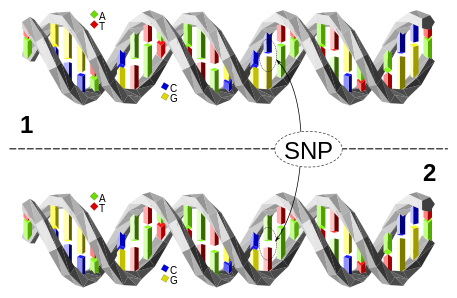
\includegraphics[width=0.8\linewidth]{images/SNP_Picture} 

}

\caption{SNP Picture}\label{fig:Snp-Pic}
\end{figure}

There are several goals to genetic mapping and association studies that
identify certain regions of the genome that contain genes involved in
specifying a quantitative trait, referred to as quantitative trait loci
(QTLs). One main goal is to estimate the genetic effects of these loci.
The relationship between the genetic effects of QTLs and the phenotypic
value of quantitative traits can be described by a linear model
(\cite{collard2005introduction}, \cite{xu2007empirical}). Typically,
because of the high throughput nature of the data there are a large
number of markers across the whole genome, and most of the markers may
have very little or next no effect on the phenotype under study. The
models can be very sparse, with most cases, the number of genetic
markers or variables is bigger than the sample size, especially when
interactions among markers are considered. This makes a model is over
saturated and further model selection techniques may be required to
capture the necessary information. \cite{dong2015accurate}

\begin{figure}

{\centering 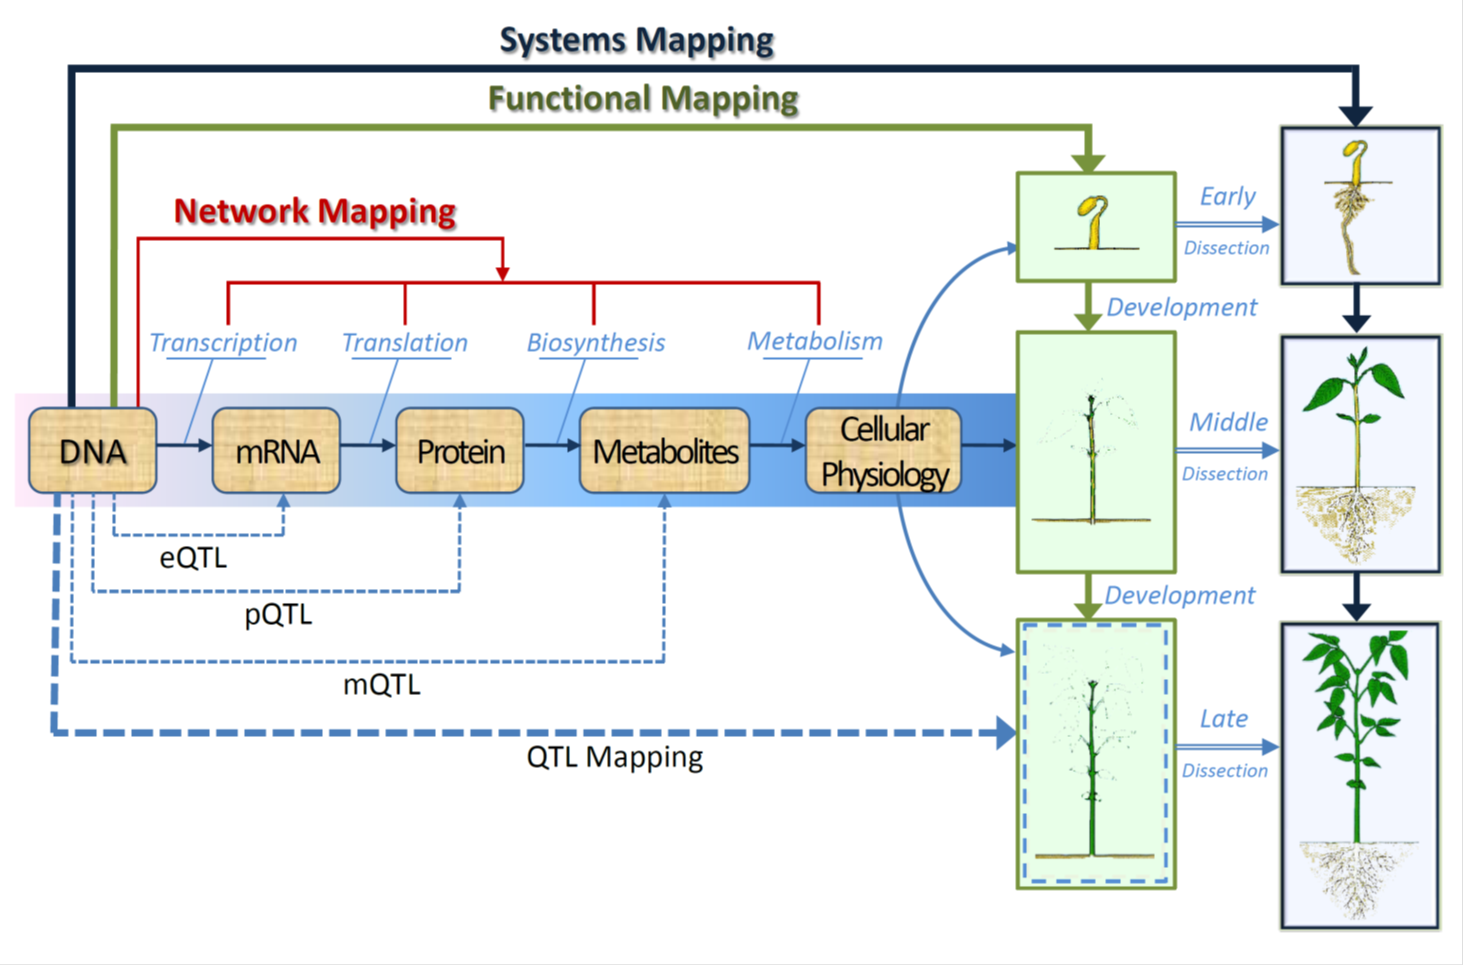
\includegraphics[width=0.8\linewidth]{images/SystemsMapping} 

}

\caption{Systems Map}\label{fig:system-map}
\end{figure}

\section{Some Exisiting Methods}\label{some-exisiting-methods}

Numerous methods exist and are being developed to measure and find
quantitative trait loci (QTL) effects. These methods can broadly fall
into three main categories. These categories are Least-Square methods,
maximum likelihood and Bayesian approaches. (\cite{wu2007statistical})
Each method has advantages and considerations that you would need to be
aware before conducting analyses to find QTL effects from the given
markers. A brief discussions on a few of the methods are given to
highlight some areas of consideration and how the methods proposed can
handle such considerations.

Marker Regression would fall in the category of Least Squares
approaches. If looking at one marker analysis general t-test and ANOVA
procedures can be used to analyze the relationship. It is not
recommended however for use in general practice because you do not know
how dense the markers are measured. QTL interval mapping would be
preferred in such an analysis because the methods take account for
missing genotype data that may not have been measured. When estimating a
QTL position through maximum likelihood methods, like interval mapping,
positions of other possible QTLs could affect the detection of the true
position. Neighboring QTLs could possibly flatten the likelihood in
instances where there are multiple QTLs on the same chromosome. This
would make an effect look less significant at a given location than it
actually is. Another possibility is that in the search over the interval
you may find an area where the likelihood could reach a peak but could
be a ``ghost'' QTL. This is where an effect is observed because a
neighboring QTL is skewing the results at the particular position you
are looking in and the result is a false discovery of the position.
Marker Regression has been shown to improve interval mapping, which is
call Composite Interval Mapping. This is where the QTL position found is
also combined in a linear regression where the covariates are the other
markers in the dataset. By including the markers as covariates the other
position in the chromosome are accounted for in the analysis and false
discovery is reduced.

The analysis of interval mapping and single marker analyses has shown to
be effective but it limits our inference to one marker at a time as a
possible loci that controls a trait. Using Marker Regression however you
can incorporate multiple markers in a single analysis to test for
possible QTL for a given trait. It is cautioned that running such an
analysis is only an approximate test because the null hypothesis is
there is no difference between the marker levels and therefore a
non-mixture distribution but the alternative is a mixture of
distributions. The assumptions regression would make of the errors
within the marker type to be normally distributed may not be entirely
met if the QTL's fall between the marker regions. However
\cite{whittaker1996mapping} have shown that a direct regression of
phenotypes on marker types, provides the same information about location
of QTL-effects without having to step to all positions on the interval.
With this information using the entire marker set in a regression
analysis would provide a nice, computationally efficient way to map out
the genetic architecture of a trait.

\section{Chapter Overview}\label{chapter-overview}

The main theme of this paper is to propose an improvements on selection
procedures which use regression techniques to approach high dimensional
variable selection such as the ones arising in epistatic analysis. The
variable selection procedure for QTL mapping can be seen as one of
deciding which subset of variables have effects on the phenotypes of
interest, and identifying those specific traits out of all possible
effects between the markers. Each procedure proposed is a forward
selecting method that starts with the empty set. After starting with the
empty set each procedure continues to add markers to the model set as
possible QTLs. Once a designated stopping criteria is met the final
model is fit and the effects are estimated. Each of the next three
chapters focuses on a new selection procedure and the properties of
them.

\subsection{HighDeQTL}\label{highdeqtl}

In this chapter we introduce the iform procedure, originally proposed by
(\cite{hao2014interaction}). Included in the chapter is the algorithm
and how it compares to forward selection. From there it is adapted to
use for a genetic mapping studies. The properties of this will be
explored in detail. Simulation studies were conducted to assess how well
the properties are met and under what conditions. Comparisons to other
models was also explored to get a sense of the utility and advantages
that come with the new selection procedure. After the comparisons and
simulations a real world application is performed. The application was a
reanalysis of a data set using C Elegans first proposed by
\cite{rockman2010selection}.

\subsection{Higher Order Epistasis}\label{higher-order-epistasis}

The next chapter considers higher order epistasis and its importance.
Currently it is under studied because of practical limitations not
because of biological limitations or relevance. The iFORM procedure
proposed in Chapter 2 is then extended to incorporate higher orders of
epistatic effects. Even though similar methods are being used the
properties are still studied and assessed. Simulation studies were
performed to assess practical applications. Several scenarios and
comparison models were considered to extensively look at what properties
were being met and which were not. Then an application to Mei tree
growth was conducted in order to see the real world application of such
a selection procedure. Different growth parameters were previously fit
and these were used as the phenotype. Interesting and more predictive
implications came out of the model when considering higher order
epistasis throughout the selection procedure.

\subsection{iForm Funcional Mapping}\label{iform-funcional-mapping}

The application of the Mei tree growth led into exploring to use a more
functional phenotype as a response throughout the selection procedure.
In order to use all relevant information of the repeated measure data,
it would take an additional computation burden to the selection and the
modeling but it would also give more power and flexibility to the
modeling that would not be present otherwise. It is important to use all
relevant information in order to make the most accurate prediction about
the data. Using a growth curve model to assist in fitting the data would
help ease some of the computational burden. The selection of genetic
effects however would be very simplistic as some additive shift to the
curve. This view may not be the most accurate and therefore more
complicated structures will be implemented to produce better results.
Legendre orthogonal polynomials were considered to model the genetic
effects. These polynomials have various forms and would allow for the
genetic effect to follow different patterns but also not induce
unnecessary correlation between predictors when included in the model.
Again, simulation studies were conducted and a reanalysis of the full
Mei tree dataset was considered.

\subsection{Conclusions}\label{conclusions}

Finally in the last chapter it will focus on comparisons and discussion
around the models proposed. Future aims of the research goals will be
explored also. Seeing how my current research will lead into the aims
and what possible directions can be explored with the given statistical
frameworks.

\chapter{High Dimensional eQTL}\label{highdeqtl}

\chapter{High-order Epistatic Networks}\label{highorder}

\chapter{iForm Functional Mapping}\label{iformfunc}

\chapter{Conclusions}\label{conclusions-1}

\chapter{Appendix}\label{appendix}

\chapter{Placeholder}\label{placeholder}

\bibliography{packages.bib,book.bib}
\addcontentsline{toc}{chapter}{\bibname}


\end{document}
=======
\documentclass[11pt,]{book}
\usepackage{lmodern}
\usepackage{setspace}
\setstretch{2}
\usepackage{amssymb,amsmath}
\usepackage{ifxetex,ifluatex}
\usepackage{fixltx2e} % provides \textsubscript
\ifnum 0\ifxetex 1\fi\ifluatex 1\fi=0 % if pdftex
  \usepackage[T1]{fontenc}
  \usepackage[utf8]{inputenc}
\else % if luatex or xelatex
  \ifxetex
    \usepackage{mathspec}
  \else
    \usepackage{fontspec}
  \fi
  \defaultfontfeatures{Ligatures=TeX,Scale=MatchLowercase}
\fi
% use upquote if available, for straight quotes in verbatim environments
\IfFileExists{upquote.sty}{\usepackage{upquote}}{}
% use microtype if available
\IfFileExists{microtype.sty}{%
\usepackage{microtype}
\UseMicrotypeSet[protrusion]{basicmath} % disable protrusion for tt fonts
}{}
\usepackage[margin=1in]{geometry}
\usepackage{hyperref}
\hypersetup{unicode=true,
            pdfborder={0 0 0},
            breaklinks=true}
\urlstyle{same}  % don't use monospace font for urls
\usepackage{natbib}
\bibliographystyle{apalike}
\usepackage{longtable,booktabs}
\usepackage{graphicx,grffile}
\makeatletter
\def\maxwidth{\ifdim\Gin@nat@width>\linewidth\linewidth\else\Gin@nat@width\fi}
\def\maxheight{\ifdim\Gin@nat@height>\textheight\textheight\else\Gin@nat@height\fi}
\makeatother
% Scale images if necessary, so that they will not overflow the page
% margins by default, and it is still possible to overwrite the defaults
% using explicit options in \includegraphics[width, height, ...]{}
\setkeys{Gin}{width=\maxwidth,height=\maxheight,keepaspectratio}
\IfFileExists{parskip.sty}{%
\usepackage{parskip}
}{% else
\setlength{\parindent}{0pt}
\setlength{\parskip}{6pt plus 2pt minus 1pt}
}
\setlength{\emergencystretch}{3em}  % prevent overfull lines
\providecommand{\tightlist}{%
  \setlength{\itemsep}{0pt}\setlength{\parskip}{0pt}}
\setcounter{secnumdepth}{5}
% Redefines (sub)paragraphs to behave more like sections
\ifx\paragraph\undefined\else
\let\oldparagraph\paragraph
\renewcommand{\paragraph}[1]{\oldparagraph{#1}\mbox{}}
\fi
\ifx\subparagraph\undefined\else
\let\oldsubparagraph\subparagraph
\renewcommand{\subparagraph}[1]{\oldsubparagraph{#1}\mbox{}}
\fi

%%% Use protect on footnotes to avoid problems with footnotes in titles
\let\rmarkdownfootnote\footnote%
\def\footnote{\protect\rmarkdownfootnote}

%%% Change title format to be more compact
\usepackage{titling}

% Create subtitle command for use in maketitle
\newcommand{\subtitle}[1]{
  \posttitle{
    \begin{center}\large#1\end{center}
    }
}

\setlength{\droptitle}{-2em}
  \title{}
  \pretitle{\vspace{\droptitle}}
  \posttitle{}
  \author{}
  \preauthor{}\postauthor{}
  \date{}
  \predate{}\postdate{}

\usepackage{booktabs}
\usepackage{amsthm}
\usepackage[utf8]{inputenc}
\usepackage[english]{babel}
\makeatletter
\def\thm@space@setup{%
  \thm@preskip=8pt plus 2pt minus 4pt
  \thm@postskip=\thm@preskip
}
\makeatother

\addcontentsline{toc}{chapter}{\listtablename}{ix}
\addcontentsline{toc}{chapter}{\listfigurename}{xi}

\usepackage{amsthm}
\newtheorem{theorem}{Theorem}[chapter]
\newtheorem{lemma}{Lemma}[chapter]
\theoremstyle{definition}
\newtheorem{definition}{Definition}[chapter]
\newtheorem{corollary}{Corollary}[chapter]
\newtheorem{proposition}{Proposition}[chapter]
\theoremstyle{definition}
\newtheorem{example}{Example}[chapter]
\theoremstyle{remark}
\newtheorem*{remark}{Remark}
\begin{document}

\begin{center}
\begin{titlepage}
\bf{The Pennsylvania State University} \\
The Graduate School \\
College of Medicine Public Health Sciences \\

STATISTICAL MODELS FOR HIGH DIMENSIONAL SCREENING OF GENETIC AND EPIGENETIC EFFECTS

A Dissertation in \\
Biostatistics \\
by \\
Kirk Gosik \\
(c) 2017 Kirk Gosik \\

Doctor of Philosophy \\
February 2017 \\
\end{titlepage}
\newpage
\pagenumbering{roman}
\setcounter{page}{2}
The dissertation of Kirk Gosik was reviewed and approved* by the following:

Rongling Wu \\
Distinguished Professor of Public Health Sciences and Statistics \\
Thesis Advisor, Chair of Committee

Vernon Chinchilli \\
Distinguished Professor and Chair of Public Health Sciences


Lan Kong \\
Associate Professor of Public Health Sciences

James Broach \\
Distinguished Professor and Chair of Biochemistry and Molecular Biology \\


\newpage

Abstract

Knowledge about how changes in gene expression are encoded by expression quantitative trait loci (eQTLs) is a key to construct the genotype-phenotype map for complex traits or diseases. Traditional eQTL mapping is to associate one transcript with a single marker at a time, thereby limiting our inference about a complete picture of the genetic architecture of gene expression. Here, I present innovative applications of variable selection approaches to systematically detect main effects and interaction effects among all possible loci on differentiation and function of gene expression and other phenotypes of interest. Forward-selection-based procedures were particularly implemented to tackle complex covariance structures of gene-gene interactions. Simulation studies were performed on each of the models to assess the computational properties of each model.  Applications of the models were also performed on real datasets.  The first was a reanalysis of a published genetic and genomic dataset collected in a mapping population of Caenorhabditis elegans, gaining new discoveries on the genetic origin of gene expression differentiation, which could not be detected by a traditional one-locus/one-transcript analysis approach.  The next dataset was of Mei Tree growth, analyzing the genetic control of the height and diameter during the developmental process.  The underlying genotypes and epistasis that impact the process of these developments were considered as candidates for the selection of the procedure.

\end{center}

{
\setcounter{tocdepth}{1}
\tableofcontents
}
\listoftables
\listoffigures
\chapter{Introduction}\label{intro}

\pagenumbering{arabic} \setcounter{page}{1}

\section{Background}\label{background}

There are several techniques used for studying genetics and mapping the
results. Some of the more popular techniques include cross-breeding
experiments or, in the case of humans, the examination of family
histories, known as pedigrees. More recently, CRISPR/Cas9 can be used to
mimic mitotic recombination to help map out genes as well.
(\cite{sadhu2016crispr})

Construction of genetic maps are a variety of techniques used to show
relative positions between genes or other sequence features of the
genome and the phenotype that is controlled by such sequences. Genes are
very useful markers but they are by no means ideal. One problem,
especially with larger genomes such as those of vertebrates and
flowering plants, is that a map based entirely on genes is not very
detailed.(\cite{brown2006genomes}) Genes have long areas of non-coding
regions between them and therefore result in large gaps from gene to
gene. This is further complicated because not every gene has allelic
forms that can be easily or conveniently distinguished. With these
considerations in mind gene maps may not be comprehensive enough and
other markers may be needed.

According to brown, mapped features that are not genes are called DNA
markers. As with gene markers, a DNA marker must have at least two
alleles to be useful. There are three types of DNA sequence feature that
satisfy this requirement: restriction fragment length polymorphisms
(RFLPs), simple sequence length polymorphisms (SSLPs), and single
nucleotide polymorphisms (SNPs). (\cite{brown2006genomes}) The genetic
markers that have been emphasized in this work are single nucleotide
polymorphisms. Attempting to be at the highest levels of resolution for
identifying quantitative traits, using SNPs are the most specific case.
This will give exact location of the nucleotide that may be impacting
the genetic control over the phenotype.

\begin{figure}

{\centering 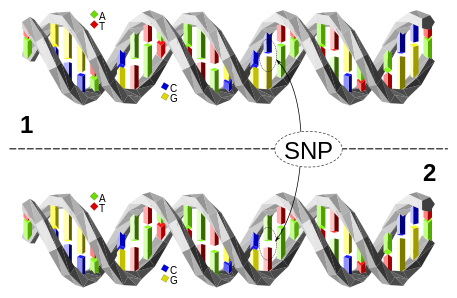
\includegraphics[width=0.8\linewidth]{images/SNP_Picture} 

}

\caption{SNP Picture}\label{fig:Snp-Pic}
\end{figure}

There are several goals to genetic mapping and association studies that
identify certain regions of the genome that contain genes involved in
specifying a quantitative trait, referred to as quantitative trait loci
(QTLs). One main goal is to estimate the genetic effects of these loci.
The relationship between the genetic effects of QTLs and the phenotypic
value of quantitative traits can be described by a linear model
(\cite{collard2005introduction}, \cite{xu2007empirical}). Typically,
because of the high throughput nature of the data there are a large
number of markers across the whole genome, and most of the markers may
have very little or next no effect on the phenotype under study. The
models can be very sparse, with most cases, the number of genetic
markers or variables is bigger than the sample size, especially when
interactions among markers are considered. This makes a model is over
saturated and further model selection techniques may be required to
capture the necessary information. \cite{dong2015accurate}

\begin{figure}

{\centering 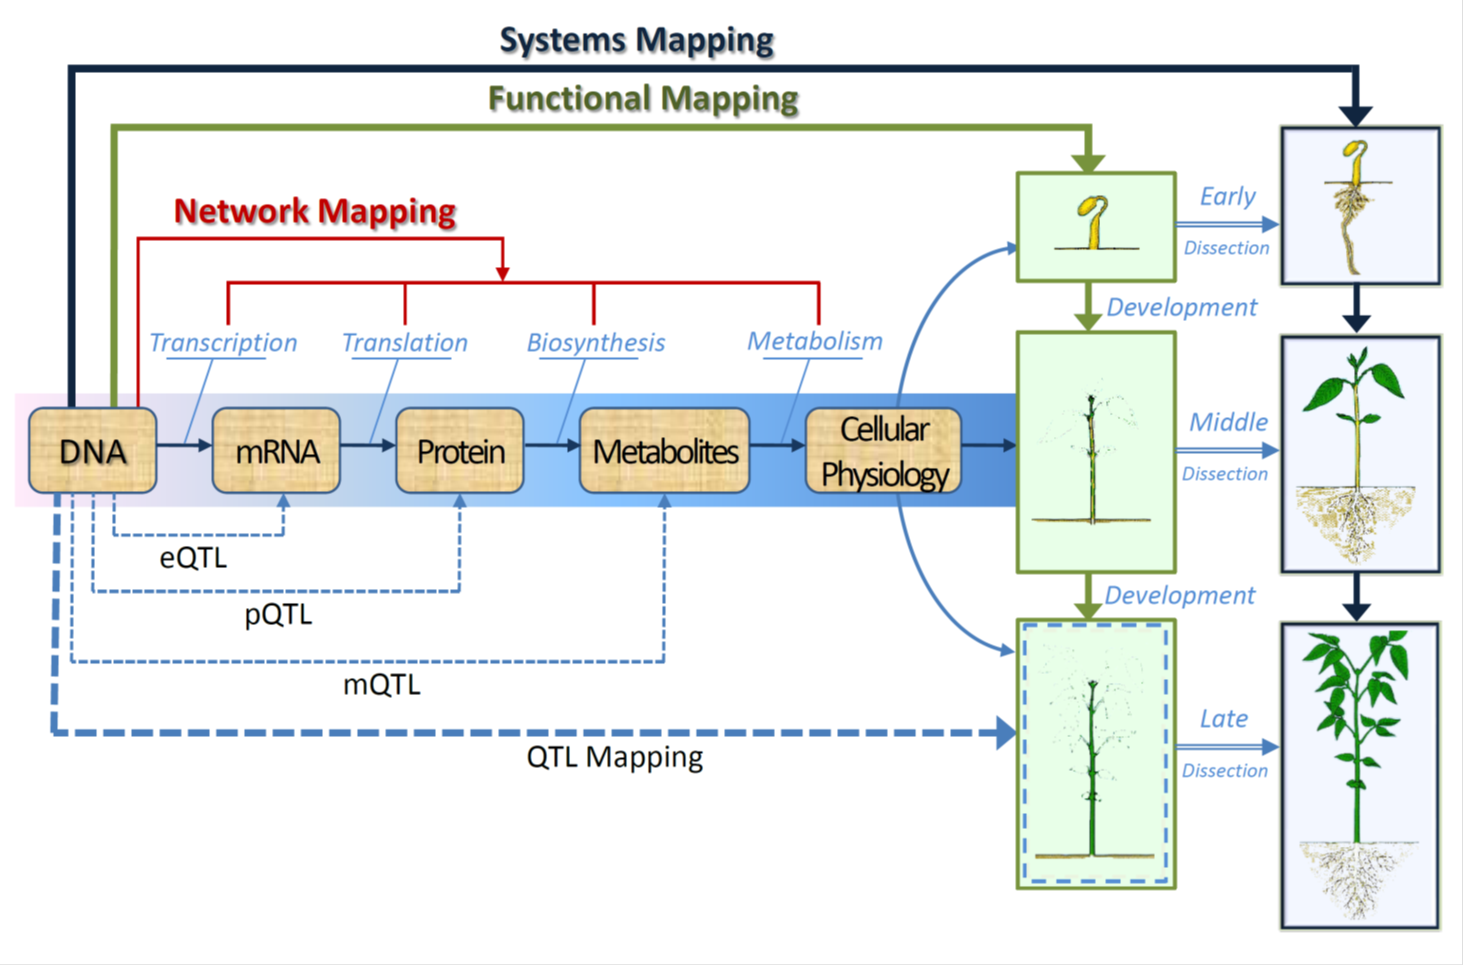
\includegraphics[width=0.8\linewidth]{images/SystemsMapping} 

}

\caption{Systems Map}\label{fig:system-map}
\end{figure}

\section{Some Exisiting Methods}\label{some-exisiting-methods}

Numerous methods exist and are being developed to measure and find
quantitative trait loci (QTL) effects. These methods can broadly fall
into three main categories. These categories are Least-Square methods,
maximum likelihood and Bayesian approaches. (\cite{wu2007statistical})
Each method has advantages and considerations that you would need to be
aware before conducting analyses to find QTL effects from the given
markers. A brief discussions on a few of the methods are given to
highlight some areas of consideration and how the methods proposed can
handle such considerations.

Marker Regression would fall in the category of Least Squares
approaches. If looking at one marker analysis general t-test and ANOVA
procedures can be used to analyze the relationship. It is not
recommended however for use in general practice because you do not know
how dense the markers are measured. QTL interval mapping would be
preferred in such an analysis because the methods take account for
missing genotype data that may not have been measured. When estimating a
QTL position through maximum likelihood methods, like interval mapping,
positions of other possible QTLs could affect the detection of the true
position. Neighboring QTLs could possibly flatten the likelihood in
instances where there are multiple QTLs on the same chromosome. This
would make an effect look less significant at a given location than it
actually is. Another possibility is that in the search over the interval
you may find an area where the likelihood could reach a peak but could
be a ``ghost'' QTL. This is where an effect is observed because a
neighboring QTL is skewing the results at the particular position you
are looking in and the result is a false discovery of the position.
Marker Regression has been shown to improve interval mapping, which is
call Composite Interval Mapping. This is where the QTL position found is
also combined in a linear regression where the covariates are the other
markers in the dataset. By including the markers as covariates the other
position in the chromosome are accounted for in the analysis and false
discovery is reduced.

The analysis of interval mapping and single marker analyses has shown to
be effective but it limits our inference to one marker at a time as a
possible loci that controls a trait. Using Marker Regression however you
can incorporate multiple markers in a single analysis to test for
possible QTL for a given trait. It is cautioned that running such an
analysis is only an approximate test because the null hypothesis is
there is no difference between the marker levels and therefore a
non-mixture distribution but the alternative is a mixture of
distributions. The assumptions regression would make of the errors
within the marker type to be normally distributed may not be entirely
met if the QTL's fall between the marker regions. However
\cite{whittaker1996mapping} have shown that a direct regression of
phenotypes on marker types, provides the same information about location
of QTL-effects without having to step to all positions on the interval.
With this information using the entire marker set in a regression
analysis would provide a nice, computationally efficient way to map out
the genetic architecture of a trait.

\section{Chapter Overview}\label{chapter-overview}

The main theme of this paper is to propose an improvements on selection
procedures which use regression techniques to approach high dimensional
variable selection such as the ones arising in epistatic analysis. The
variable selection procedure for QTL mapping can be seen as one of
deciding which subset of variables have effects on the phenotypes of
interest, and identifying those specific traits out of all possible
effects between the markers. Each procedure proposed is a forward
selecting method that starts with the empty set. After starting with the
empty set each procedure continues to add markers to the model set as
possible QTLs. Once a designated stopping criteria is met the final
model is fit and the effects are estimated. Each of the next three
chapters focuses on a new selection procedure and the properties of
them.

\hypertarget{highdeqtl}{\subsection{HighDeQTL}\label{highdeqtl}}

In this chapter we introduce the iform procedure, originally proposed by
(\cite{hao2014interaction}). Included in the chapter is the algorithm
and how it compares to forward selection. From there it is adapted to
use for a genetic mapping studies. The properties of this will be
explored in detail. Simulation studies were conducted to assess how well
the properties are met and under what conditions. Comparisons to other
models was also explored to get a sense of the utility and advantages
that come with the new selection procedure. After the comparisons and
simulations a real world application is performed. The application was a
reanalysis of a data set using C Elegans first proposed by
\cite{rockman2010selection}.

\subsection{Higher Order Epistasis}\label{higher-order-epistasis}

The next chapter considers higher order epistasis and its importance.
Currently it is under studied because of practical limitations not
because of biological limitations or relevance. The iFORM procedure
proposed in Chapter 2 is then extended to incorporate higher orders of
epistatic effects. Even though similar methods are being used the
properties are still studied and assessed. Simulation studies were
performed to assess practical applications. Several scenarios and
comparison models were considered to extensively look at what properties
were being met and which were not. Then an application to Mei tree
growth was conducted in order to see the real world application of such
a selection procedure. Different growth parameters were previously fit
and these were used as the phenotype. Interesting and more predictive
implications came out of the model when considering higher order
epistasis throughout the selection procedure.

\subsection{iForm Funcional Mapping}\label{iform-funcional-mapping}

The application of the Mei tree growth led into exploring to use a more
functional phenotype as a response throughout the selection procedure.
In order to use all relevant information of the repeated measure data,
it would take an additional computation burden to the selection and the
modeling but it would also give more power and flexibility to the
modeling that would not be present otherwise. It is important to use all
relevant information in order to make the most accurate prediction about
the data. Using a growth curve model to assist in fitting the data would
help ease some of the computational burden. The selection of genetic
effects however would be very simplistic as some additive shift to the
curve. This view may not be the most accurate and therefore more
complicated structures will be implemented to produce better results.
Legendre orthogonal polynomials were considered to model the genetic
effects. These polynomials have various forms and would allow for the
genetic effect to follow different patterns but also not induce
unnecessary correlation between predictors when included in the model.
Again, simulation studies were conducted and a reanalysis of the full
Mei tree dataset was considered.

\subsection{Conclusions}\label{conclusions}

Finally the last chapter will focus on comparisons and discussion around
the models proposed. It will also summarize and discuss advantages to
each of the proposed models. What benefits and looks to be aware of will
also be identified. Future aims of the research goals will be explored
following the discussion. The possible directions the research can be
taken and also some extensions that are possible. Finally, seeing how my
current research will lead into the aims and what possible directions
can be explored with the given statistical frameworks will be dicussed.

\hypertarget{highdeqtl}{\chapter{High Dimensional
eQTL}\label{highdeqtl}}

\section{Motivation}\label{motivation}

Since activation or inhibition of gene expression causes change in
phenotypic formation, the identification of expression quantitative
trait loci (eQTLs) that regulate the pattern of gene expression is
essential for constructing a precise genotype-phenotype map
(\cite{emilsson2008genetics}; \cite{cookson2009mapping};
\cite{nica2013expression}). With the advent and development of various
biotechnologies, it has become possible that genome-scale marker and
expression data can be generated, providing an important fuel to
systematically study the biological function of any types of cellular
components in an organism (\cite{kim2014meta}; \cite{fairfax2014innate};
\cite{lee2014common}). Several genome-wide association studies (GWAS)
have been initiated to map a complete set of eQTLs for the abundance of
genome-wide transcripts whose expression levels are related to
biological or clinical traits
(\cite{nica2013expression};\cite{li2013using};
\cite{koopmann2014genome}). Statistical analysis and modeling are
playing an increasing role in mapping and identifying the underlying
eQTLs from massive amounts of observed data
(\cite{kendziorski2006statistical}; \cite{chun2009expression};
\cite{sun2012statistical}; \cite{flutre2013statistical}).

A typical eQTL mapping approach is to associate a gene transcript with a
single marker such as single nucleotide polymorphism (SNP). By analyzing
the significance of all these markers one by one adjusted for multiple
testing, one can count significant loci that contribute to variation of
expression by the gene. This marginal approach based on a simple
regression model has been instrumental for the identification of eQTLs
in a variety of organisms (\cite{rockman2010selection};
\cite{kim2014meta}). However, there are two major limitations for the
results by such a marginal analysis: First, it does not take into
account the dependence of different markers, thus a significant
association detected by one marker may be due to the other markers that
are linked with it. The marginal marker analysis cannot separate the
confounding effect of eQTLs due to marker-marker dependence or linkage
(\cite{wu2007statistical}). Second, an eQTL may act through its
interaction with other eQTLs and environmental factors. Because of their
paramount importance in affecting complex diseases and traits, gene-gene
interactions, or epistatic effects, and gene-environment interactions
have been studied intensively in modern biological and medical research
(\cite{cheverud1995epistasis}; \cite{moore2003ubiquitous};
\cite{van2010detection}; \cite{mackay2014epistasis})

These two limitations can be overcome by analyzing all markers and their
pairwise interactions simultaneously through formulating a
high-dimensional regression model. Although it can infer a complete
picture of the genetic architecture of gene expression, this endeavor is
highly challenged by the curse of dimensionality, i.e., the number of
predictors far exceeds the number of observations. The past decade has
witnessed the tremendous development of variable selection models for
high-dimensional data analysis, such as LASSO
(\cite{tibshirani1996regression}), SCAD (\cite{fan2001variable}),
Dantzig selector (\cite{candes2007dantzig}), elastic net
(\cite{zhao2006model}), minimax concave penalty (MCP)
(\cite{zhang2010nearly}) among others. Many methods possess favorable
theoretical properties such as model selection consistency
(\cite{zhao2006model}) and oracle properties (Fan and Lv 2011). When the
number of predictors is much larger than the number of observation, sure
screening is a more realistic goal to achieve than oracle properties or
selection consistency (\cite{fan2008sure}; \cite{wang2009forward}). Sure
screening assures that all important variables are identified with a
probability tending to one, hence achieving effective dimension
reduction without information loss and providing a reasonable starting
point for low-dimensional methods to be applied.

More recently, Hao and Zhang (\cite{hao2014interaction}) extended
variable selection approaches to jointly model main and interaction
effects from high-dimensional data. Based on a greedy forward approach,
their model can identify all possible interaction effects through two
algorithms iFORT and iFORM which have been proved to possess sure
screening property in an ultrahigh-dimensional setting. In this article,
we implement and reform Hao and Zhang's model to map the genetic
architecture of eQTL actions and interactions for gene expression
profiles. This model is modified to accommodate to the feature of a
genetic mapping or GWAS design in which molecular markers as genetic
predictors are discrete although some additional continuous predictors
can also be considered. We expand Hao and Zhang's regression model to
include discrete components. Also, for an F2 or a natural population
with three genotypes at each locus, we need to estimate a total of eight
genetic effects for a pair of markers, which are additive and dominant
effects at each locus, and additive x additive, additive x dominant,
dominant x additive and dominant x dominant effects between the two loci
(\cite{kempthorne1968correlation}). Thus, if the number of markers is p,
a total number of predictors including all main and two-way interaction
terms is \(2p^2\). For a typical moderate-sized mapping study, in which
several thousands of markers are genotyped on a few hundred individuals,
consideration of pair-wise genetic interactions will quickly make the
dimension of predictors an ultrahigh one.

By modeling all markers jointly at one time under an organizing
framework, the modified model can detect all possible significant eQTLs
and their epistasis. An eQTL can be either a cis-QTL, coming from the
same physical location as the gene expression, or a trans-QTL, coming
from other areas of the genome. Our model can more precisely discern
these two different types of eQTLs and their interactions than
traditional marginal analysis. By reanalyzing a published data collected
in a mapping population of C. elegans (\cite{rockman2010selection}), the
new model has validated previous results by the marginal approach,
meanwhile obtained new discoveries on the genetic origin of gene
expression differentiation, which could not be detected in a traditional
way.

\section{Methods}\label{methods}

\subsection{Experimental design}\label{experimental-design}

Consider an experimental population for genetic studies of complex
traits, such as the backcross and F2 initiated from two inbred lines,
full-sib family derived from two outcrossing parents, or random samples
drawn from a natural population. These types of populations are used
specifically for different species. Although they have different levels
of complexities for statistical modeling, the genetic dissection of
different populations underlies a similar principle. For the purpose of
simplicity, we consider a backcross design in which there are only two
genotypes at each marker.

Suppose the backcross contains n progeny, each of which is genotyped by
p markers, such as single nucleotide polymorphisms (SNPs), distributed
over different chromosomes. The number of SNPs p should be large enough
to completely cover the entire genome at an adequate depth so that we
can possibly capture all possible genetic variants. An increasing body
of evidence suggests that significant SNPs associated with complex
traits or diseases are more likely to be eQTLs (\cite{li2013using}).
Hence the identification of eQTLs is an important first step toward the
genetic dissection of end-point phenotypes. For this reason, we assume
that genome-wide gene transcripts have been available for the assumed
study population. Assume that all progeny are recorded for the same
organ by microarray, leading to expression abundance data of m gene
transcripts. We purport to identify all possible genetic variants
including main effects and interaction effects of SNPs that contribute
to each gene transcript.

\subsection{Adaptation of iFORM
procedure}\label{adaptation-of-iform-procedure}

Hao and Zhang \cite{hao2014interaction} formulated an interaction
forward selecting procedure under the marginality principle (iFORM). The
marker and gene transcript data of the study population can be denoted
as \((X_i,Y_i) (i = 1,\dots, n)\) which are independent and identically
distributed copies of (X,Y), where \(X = (X_1,\dots,X_p )^T\) is a
p-dimensional predictor vector and Y is the response, expressed by a
linear regression model:

\begin{equation}
Y = \beta_0 + \beta_1 X_1 + \dots + \beta_p X_p + \epsilon
\label{eq:lin-mod}
\end{equation}

The \(\beta\)'s are the coefficients for the genetic effects of each
marker. Like most genome-wide datasets, the number of markers here
grossly outnumbers the number of observations, \(p >> n\). Therefore,
selection procedures would need to be implemented in order to fit a
linear regression model such as \eqref{eq:lin-mod}. We are already at the
point of high-dimensional data but if we want to include epistatic
effects between different markers as predictors as well it would
increase the amount of predictors by \((p^2+p)/2\) . The resulting
linear model would grow to be,

\begin{equation}
Y = \beta_0 + \beta_1 X_1 + \dots + \beta_p X_p + \gamma_{11} X_1^2 +\gamma_{12} {X_1}{X_2} + \dots + \gamma_{pp} X_p^2 + \epsilon
\label{eq:lin-mod2}
\end{equation}

where \(\gamma\)'s are the coefficients for the epistatic effects for
all the quadratic and two-way interactions between the markers. For
convenience we will assume that the markers and the transcripts are
standardized before running the selection procedure. Therefore,
\(E(X_ij )=0\), \(Var(X_ij )=1\), \(E(Y_i )=0\) and \(Var(Y_i )=1\) for
\(i=1,\dots,n\); \(j=1,\dots,p\). Also, the quadratic and two-way
interaction effects will be centered which we will write as
\(Z_i=(\dots,X_{ik} X_{il}-E(X_{ik} X_{il} ),\dots)^T\). By doing so we
would eliminate the need for an intercept in regression model
\eqref{eq:lin-mod2}. This would reduce the model to the form,

\begin{equation}
Y = X^T \beta + Z^T \gamma + \epsilon
\label{eq:lin-mod3}
\end{equation}

Some notations that will be used to define the elements of
\cite{hao2014interaction} iFORM procedure are as follows.\\
\(P_1 = {1,2,\dots,p}\) \(P_2 = {(k,l):1 \le k \le l \le p}\). which are
the index sets for the linear and two-way interactions terms,
respectively. The significant main effects for the markers and their
interaction effects are
\(\mathcal{T}_1 = {j:\beta_j \ne 0,j\in P_1},\mathcal{T}_2 = {(j,k):\beta_{jk} \ne 0,(j,k) \in P_2}\).
For any model M, \(|\mathcal{M}|\) will be used to denote the number of
predictors contained in the model. The true model size would be
indicated by \(|\mathcal{T}_1| = p_0\) and \(|\mathcal{T}_2| = q_0\) or
together would be \(|\mathcal{T}|=d_0=p_0+q_0\). For the procedure,
three sets will be used throughout. The sets are M for the model set, C
for the candidate set of predictors and S for the solution set of
predictors currently selected in the model.

There are two principles that are used in the selection procedure when
considering interactions as candidates for selection into the final
model. The first is considering the principle of marginality. The
principle states that it is inappropriate to model interaction terms
when the main effects contributing to the interaction have either not
been included in the model or are deleted because their effects become
marginal by the inclusion of the interaction effect. The second
principle important to the procedure is the heredity principle. The
strong case of the principle states that an interaction effect should
not be considered unless both the contributing main effects are in the
model (\cite{zhao2006model}). This would translate to
\(\gamma_{jk} \ne 0\) only if
\(\beta_j, \beta_k \ne 0 \forall 1 ≤ j, k ≤ p\) for model
(\eqref{eq:lin-mod2}). By including both principles during the selection
process it allows for dynamically including both main effects and
interactions effects. The interaction effects can only be considered
between the main effects currently selected into the solution set of the
model according the discussed principles. A more formal description of
the procedure is given below.

\subsection{iFORM}\label{iform}

\cite{hao2014interaction} formulated an interaction forward selecting
procedure under the marginality principle (iFORM). The procedure's
initial step starts with the empty set for both the solution set and the
model set, \(S_0=\emptyset\) and \(M_0=\emptyset\). The candidate set
contains all main effects at the beginning, \(\mathcal{C}_0 = P_1\), for
each of the markers as a possible eQTL. Typical forward selection
procedures are carried out to start the selection. Each marker is tested
individually using a marker regression. The marker that results in the
lowest residual sum of squares is the marker selected from the candidate
set into the solution set as an eQTL. This is then iterated again for a
selection of another marker into the model set. Once there are at least
two main effects selected into the solution set, using the strong
heredity principle, the quadratic and two-way interactions are then
created and placed into the candidate set as possible eQTLs for
selection in the next step. This process continues selecting main
effects or the newly created interaction effects into the solution set.
If another main effect is selected into the solution set, then the
candidate set grows with the creation of all possible two-way
interactions of the main effects that are currently in the solution set.
This is continued until a designated stopping value, say d. For the
number of predictors placed into the model set from the solution set the
Bayesian information Criterion was used,
\(BIC_2(\hat{\mathcal{M}})=log(\hat \sigma_\hat\mathcal{M})+n^{-1} |\hat\mathcal{M}|\star(log(n)+2\star log(d^\star))\),
where \(\sigma^2_\hat{\mathcal{M}}\) is the sample variance for the
given model, \(|\hat{M}|\) is the size of the model or the number of
predictors selected into the given model, and n is the sample size. The
\(d^{\star}\) term is the number of predictors in the full model. This
was proposed as \(BIC_2\) by \cite{chen2008extended} which they derived
to help control the false discovery rate in high dimensional data
situations. They also showed that it was selection consistent if
\(d^{\star} = O(n^\xi)\) for some \(\xi \gt 0\). The only difference
between the traditional \(BIC\) calculation and the \(BIC_2\) is the
additional term involving \(2log(d*)\). Ignoring the \(BIC\), the most
the number of steps in the solution path is of size n. The parameter d
controls the overall length of the solution path. In practice, the exact
number of predictors to include, say \(d_0\), in the true model is
unknown. We want to make d large enough to include d\_0 but not so large
as to fit the model to the point where it becomes over saturated. Using
the \(BIC_2\) should help avoid such a matter as well. It is reasonable
to assume that \(d_0\) is much smaller than n in high dimensional sparse
regression problems (\cite{fan2008sure}). Since this is the case, for
the purposes of our model, d was set to be no larger than \(n/log(n)\).
Generally, the \(BIC_2\) should reach minimum, indicating the optimal
stopping point, before the designated stopping value, is reached.

\subsection{Some considerations}\label{some-considerations}

There were some considerations and pre-processing steps taken before the
iFORM procedure was implemented. The first consideration was to see if
there were any exact duplicate markers in the dataset. One drawback that
could arise with marker datasets when attempting to run multiple linear
regression is the possibility of duplicate markers in the dataset. If
two different markers would happen to have exactly the same genotypes
for each subject it would show up as an exact linear combination of each
other if both markers were to be placed in the linear model. Including
redundant markers in a linear model would not add any additional
information and therefore should not be included in the candidate set
during the selection procedure. This also reduces the dimension slightly
when there are duplicate markers in the dataset.

Another consideration made is the type of coding used for the genotypes.
At any given eQTL, the jth eQTL, say, there are two possible genotypes:
\(Q_j\) \(Q_j\) and \(Q_j\) \(q_j\), making the total number of possible
QTL genotypes in the population 2\^{}m. The goal of a genetic model is
to relate the \(2^m\) possible genotypic values to a set of genetic
parameters, such that these parameters are interpretable in terms of
main and epistatic effects of the m eQTL. A genetic model is to use
orthogonal contrast scales because it is consistent in the sense that
the effect of a eQTL is consistently defined whether the genetic model
includes one, two, three, or more eQTL (\cite{kao2002modeling}). The
orthogonal contrasts for the genetic model can be expressed by
\[x_{ij} = \left[\frac{-1}{2}~if~homozygote~Q_j Q_j, \frac{-1}{2}~if~heterozygote~Q_j q_j \right]\]
Typically in an inbred line backcross population a given genotype is
coded with a 0 and 1. However there are two draws backs to this coding
when considering the selection procedures discussed above. The first
issue comes with not including an intercept in model
(\eqref{eq:lin-mod2}). If this is the case each of the predictors would
need to be centered making the coding to \(-\frac{1}{2}\) and
\(\frac{1}{2}\) instead of 0 and 1. Besides meeting the assumptions of
the model that the predictors are centered, it is also beneficial for
the interaction effects as well. If the coding would remain at 0's and
1's, the interaction coding would also consist of 0's and 1's. This
could propose a problem because three out of the four scenarios of
epistasis between markers would result in a coding of 0 for the level in
the interaction effect. This has the potential to falsely skew the data
of no additive effect for interactions terms because of the sparseness
of coding. By centering the coding to \((-\frac{1}{2},\frac{1}{2})\), it
would result in an interaction effect being coded as
\((-\frac{1}{4},\frac{1}{4})\). This coding would happen for different
scenarios for each of the levels. The \(-\frac{1}{4}\) could arise when
the interaction is made up of a homozygote interacting with a
heterozygote genotype. A coding of \(\frac{1}{4}\) would arise by either
a homozygote interacting with another homozygote genotype, or when a
heterozygote interacts with another heterozygote genotype.

\section{Application}\label{application}

\subsection{Simulation Results}\label{simulation-results}

Simulations studies were conducted to test the theoretical properties of
the selection procedures and the results \ref{tab:sim1}, \ref{tab:sim2}
and \ref{tab:sim3}. The results were compared to several other commonly
used methods for eQTL mapping. In each of the examples the response was
generated from model (2) with σ=1,2,and 3 for the random error with a
sample size of \(n=200\). The \(X_i\)'s were all independently and
identically distributed realizations generated from \(Binomial(0.5)\)
and then orthogonal contrasts were made making each
\(x_{ij} \in (-\frac{1}{2}, \frac{1}{2})\). The true
\(\beta=(3,0,0,3,0,3,3,0_{493})\), therefore making
\(\mathcal{T}_1={1,4,6,7}\) and \(p_0=4\). The relevant interactions
were set to the pairs \(\mathcal{T}_2={(1,6),(1,7),(4,7),(4,7)}\) and
\(q_0=4\) all with \(\gamma_{jk}=3\) where \((j,k) \in \mathcal{T}_2\).
There were several methods compared during each of the simulations
\ref{tab:sim1}, \ref{tab:sim2} and \ref{tab:sim3}. The methods that were
used to model the data were single marker analysis, forward selection
involving only main effects (FS), forward selection involving all main
effects and interaction (FS2) and the iFORM procedure. Several outcomes
were evaluated to compare across each of the models. The outcomes are
separated into three parts. The first part focuses on the selection of
main effects, the second part focuses on the selection of interaction
effects and the third part is the overall model performance. Simulations
of M=100 replicates were run and the outcomes considered include

\emph{Convergence Probability (Cov)
\(\Sigma_{m=1}^MI(\mathcal{T} \subset \hat{\mathcal{T}})/M\) }Percentage
of correct zeros (Cor0)
\(\Sigma_{m=1}^M\Sigma_{j=1}^pI((\hat{\beta_j}=0,\beta_j=0)/[M(p-p_0)]\)
\emph{Percentage of incorrect zeros (Inc0)
\(\Sigma_{m=1}^M\Sigma_{j=1}^p I(\hat{\beta_j}=0,\beta_j \ne 0)/[M(p_0)]\)
}Exact Selection probability (Exact)
\(\Sigma_{m=1}^M I(\mathcal{T}=\hat{\mathcal{T}})/M\) \emph{The average
model size }Mean Square Error (MSE) \emph{Adjusted R-square }Computation
Time in seconds

In each instance of the simulation, the iFORM procedure was closest to
the simulated data, indicated as Oracle. Single marker analysis was
conducted on each of the main effects individually and the significant
markers were then designated as eQTLs. When comparing the single marker
analysis, we can see it rarely designated the full set of main effects
as significant from the simulated data. Also, no consideration for
interactions could be assessed in single marker analysis. The iFORM
procedure contains the identified main effects over 90\% of the time
across all simulations. The procedure also includes interaction
selection. The interaction screening shares a similar success rate where
the interaction effects are correctly selected over 90\% of the time as
well. Focusing on the computation time, we observed only a few seconds,
on average, increase than running single marker analysis. The final
models selected by the iFORM procedure had similar adjusted R-square
values as the Oracle results, on average. Looking at the exact selection
percentage, we can see that the vast majority of the time the correct
predictors were selected and indicated as significant each time. To
compare the interaction screening effectiveness, forward selection was
implemented on both the main effects and interactions effects. The time
it took to create the design matrix in order to implement forward
selection was not included in the computation time. As can be seen from
the results, using forward selection on the full set of main effects and
pair-wise interactions took substantially longer to run on average than
any of the other methods, including the iFORM procedure. Another
drawback to implementing forward selection on such a large set seemed to
come with over fitting the model. The selection included the maximum
number of predictors allowed by the designated stopping value and did
not use the BIC criteria for final model selection. This resulted in 19
additional predictors selected \ref{tab:sim1}, \ref{tab:sim2} and
\ref{tab:sim3}. This increased the adjusted R-square value of the final
model, however this is suspected because of over fitting the data and
not to be a true prediction of the response.

\textbf{runs off the page}

\begin{table}

\caption{\label{tab:sim1}Simulation 1 Table (sigma=1)}
\centering
\begin{tabular}[t]{lrrrrrrrrrrrr}
\toprule
Method & Cov & Cor0 & Inc0 & Exact & Cov.1 & Cor0.1 & Inc0.1 & Exact.1 & Size & MSE & X & Time\\
\midrule
Single Marker & 0.00 & 1.000 & 0.2500 & 0.00 & NA & NA & NA & NA & 3.00 & 23.630 & 0.216 & 0.824\\
FS & 0.85 & 0.953 & 0.0625 & 0.85 & NA & NA & NA & NA & 27.00 & 10.230 & 0.660 & 3.470\\
FS2 & 1.00 & 0.996 & 0.0000 & 1.00 & 0.95 & 0.981 & 0 & 0.0 & 27.00 & 0.302 & 0.989 & 72.310\\
iFORM & 0.90 & 0.999 & 0.0500 & 0.90 & 0.90 & 1.000 & 0 & 0.9 & 7.55 & 2.930 & 0.894 & 4.080\\
Oracle & 1.00 & 1.000 & 0.0000 & 1.00 & 1.00 & 1.000 & 0 & 1.0 & 8.00 & 1.023 & 0.965 & NA\\
\bottomrule
\end{tabular}
\end{table}

\begin{table}

\caption{\label{tab:sim2}Simulation 2 Table (sigma=2)}
\centering
\begin{tabular}[t]{lrrrrrrrrrrrr}
\toprule
Method & Cov & Cor0 & Inc0 & Exact & Cov.1 & Cor0.1 & Inc0.1 & Exact.1 & Size & MSE & X & Time\\
\midrule
Single Marker & 0.02 & 0.999 & 0.529 & 0.029 & NA & NA & NA & NA & 1.97 & 27.02 & 0.178 & 0.69\\
FS & 0.80 & 0.953 & 0.050 & 0.800 & NA & NA & NA & NA & 27.00 & 11.49 & 0.651 & 3.22\\
FS2 & 1.00 & 0.996 & 0.000 & 1.000 & 0.98 & 0.98 & 0 & 0.00 & 27.00 & 1.17 & 0.964 & 68.20\\
iFORM & 0.97 & 0.998 & 0.007 & 0.970 & 0.95 & 1.00 & 0 & 0.93 & 8.70 & 4.41 & 0.865 & 3.84\\
Oracle & 1.00 & 1.000 & 0.000 & 1.000 & 1.00 & 1.00 & 0 & 1.00 & 8.00 & 3.92 & 0.880 & NA\\
\bottomrule
\end{tabular}
\end{table}

\begin{table}

\caption{\label{tab:sim3}Simulation 3 Table (sigma=3)}
\centering
\begin{tabular}[t]{lrrrrrrrrrrrr}
\toprule
Method & Cov & Cor0 & Inc0 & Exact & Cov.1 & Cor0.1 & Inc0.1 & Exact.1 & Size & MSE & X & Time\\
\midrule
Single Marker & 0.00 & 0.999 & 0.612 & 0.000 & NA & NA & NA & NA & 1.65 & 33.90 & 0.138 & 0.69\\
FS & 0.82 & 0.953 & 0.043 & 0.827 & NA & NA & NA & NA & 27.00 & 14.44 & 0.633 & 3.22\\
FS2 & 1.00 & 0.997 & 0.000 & 1.000 & 0.98 & 0.97 & 0 & 0.00 & 27.00 & 2.69 & 0.931 & 68.20\\
iFORM & 0.89 & 0.995 & 0.060 & 0.896 & 0.96 & 1.00 & 0 & 0.94 & 7.93 & 11.10 & 0.713 & 3.83\\
Oracle & 1.00 & 1.000 & 0.000 & 1.000 & 1.00 & 1.00 & 0 & 1.00 & 8.00 & 8.98 & 0.771 & NA\\
\bottomrule
\end{tabular}
\end{table}

\subsection{Real Data Analysis}\label{real-data-analysis}

\cite{rockman2010selection} reported an eQTL mapping study of C. elegans
using 208 recombinant inbred advanced intercross lines (RIAIL) from a
cross between the laboratory strain, N2, and a wild isolate from Hawaii,
CB4856. Abundances of 20,000 gene transcripts were measured by
microarray in developmentally synchronized young adult hermaphrodites of
these lines, providing a genome-wide coverage of C. elegans from
WormBase, a public C. elegans genome database. The microarray data was
preprocessed through a normal--exponential convolution background
correction and normalized using quantile standardization. Although they
are closely related, the two strains used for the cross are considered
relatively divergent for C. elegans. The two strains differ roughly at
approximately 1 base pair per 900. Their RIAILs were genotyped at 1454
ordered single-nucleotide polymorphism (SNP) markers that cover the
whole genome of C. elegans including five autosomes (denoted as I -- V)
and one sex chromosome (denoted as X).

\cite{rockman2010selection} used a classic interval mapping approach to
detect 2309 eQTLs by testing and scanning associations of each SNP with
each gene transcript over the entire genome. Rockman et al's analysis
allowed a rectangular map of eQTL positions gene positions to be
constructed \ref{fig:RockmanPic} , from which one can identify cis-eQTLs
on the diagonal and trans-eQTLs off the diagonal. However, because their
association analysis was conducted individually for each SNP, the
detection of eQTLs was based on the marginal effects of individual
eQTLs, which may lead to two issues being unsolved. First, of those
eQTLs detected for the same gene transcript, some may include confounded
effects by others. Second, the effects of genetic epistasis may take
place but were not detected. By analyzing all SNPs simultaneously under
a single framework, the high-dimensional model, iFORM, implemented in
this study can more precisely characterize the genetic machinery
underlying variation in each gene transcript. More specifically, we
treat each transcript as a response with all SNP markers and their
interactions as predictors by building a big regression model.
Significant predictors were then selected based on the iFORM procedure.
A final model including both main and interaction effects can be
evaluated by calculating adjusted R-square values

\begin{figure}

{\centering 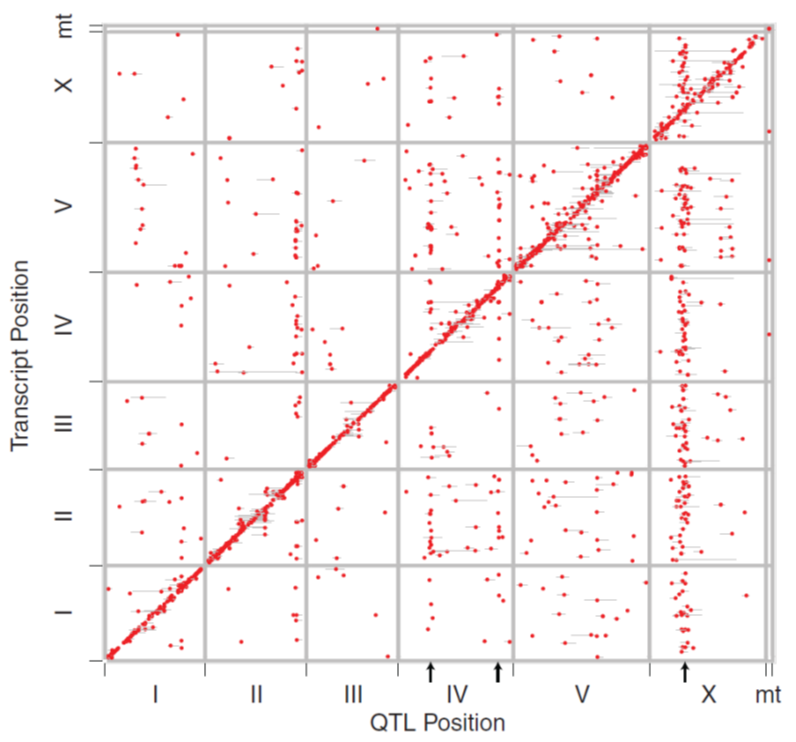
\includegraphics[width=250px,height=250px]{images/CElegansPicture} 

}

\caption{SNP Picture}\label{fig:RockmanPic}
\end{figure}

\ref{fig:ChromosomePic} illustrates the map of how a particular gene
transcript is controlled by its eQTLs through main effects and
interaction effects. For clarity of our presentation, we only chose one
representative gene transcript from each chromosome. For example, gene
transcript A\_12\_P103290 located at position 2069088 -- 2069147 of
chromosome I was detected to be controlled by main effects due to
X2\_13516256 eQTLs on chromosomes II and X4\_15632637 eQTLs on
chromosome IV and X2\_13516256:X4\_15632637 interactions between some of
these eQTLs on these two chromosomes.

\begin{figure}

{\centering 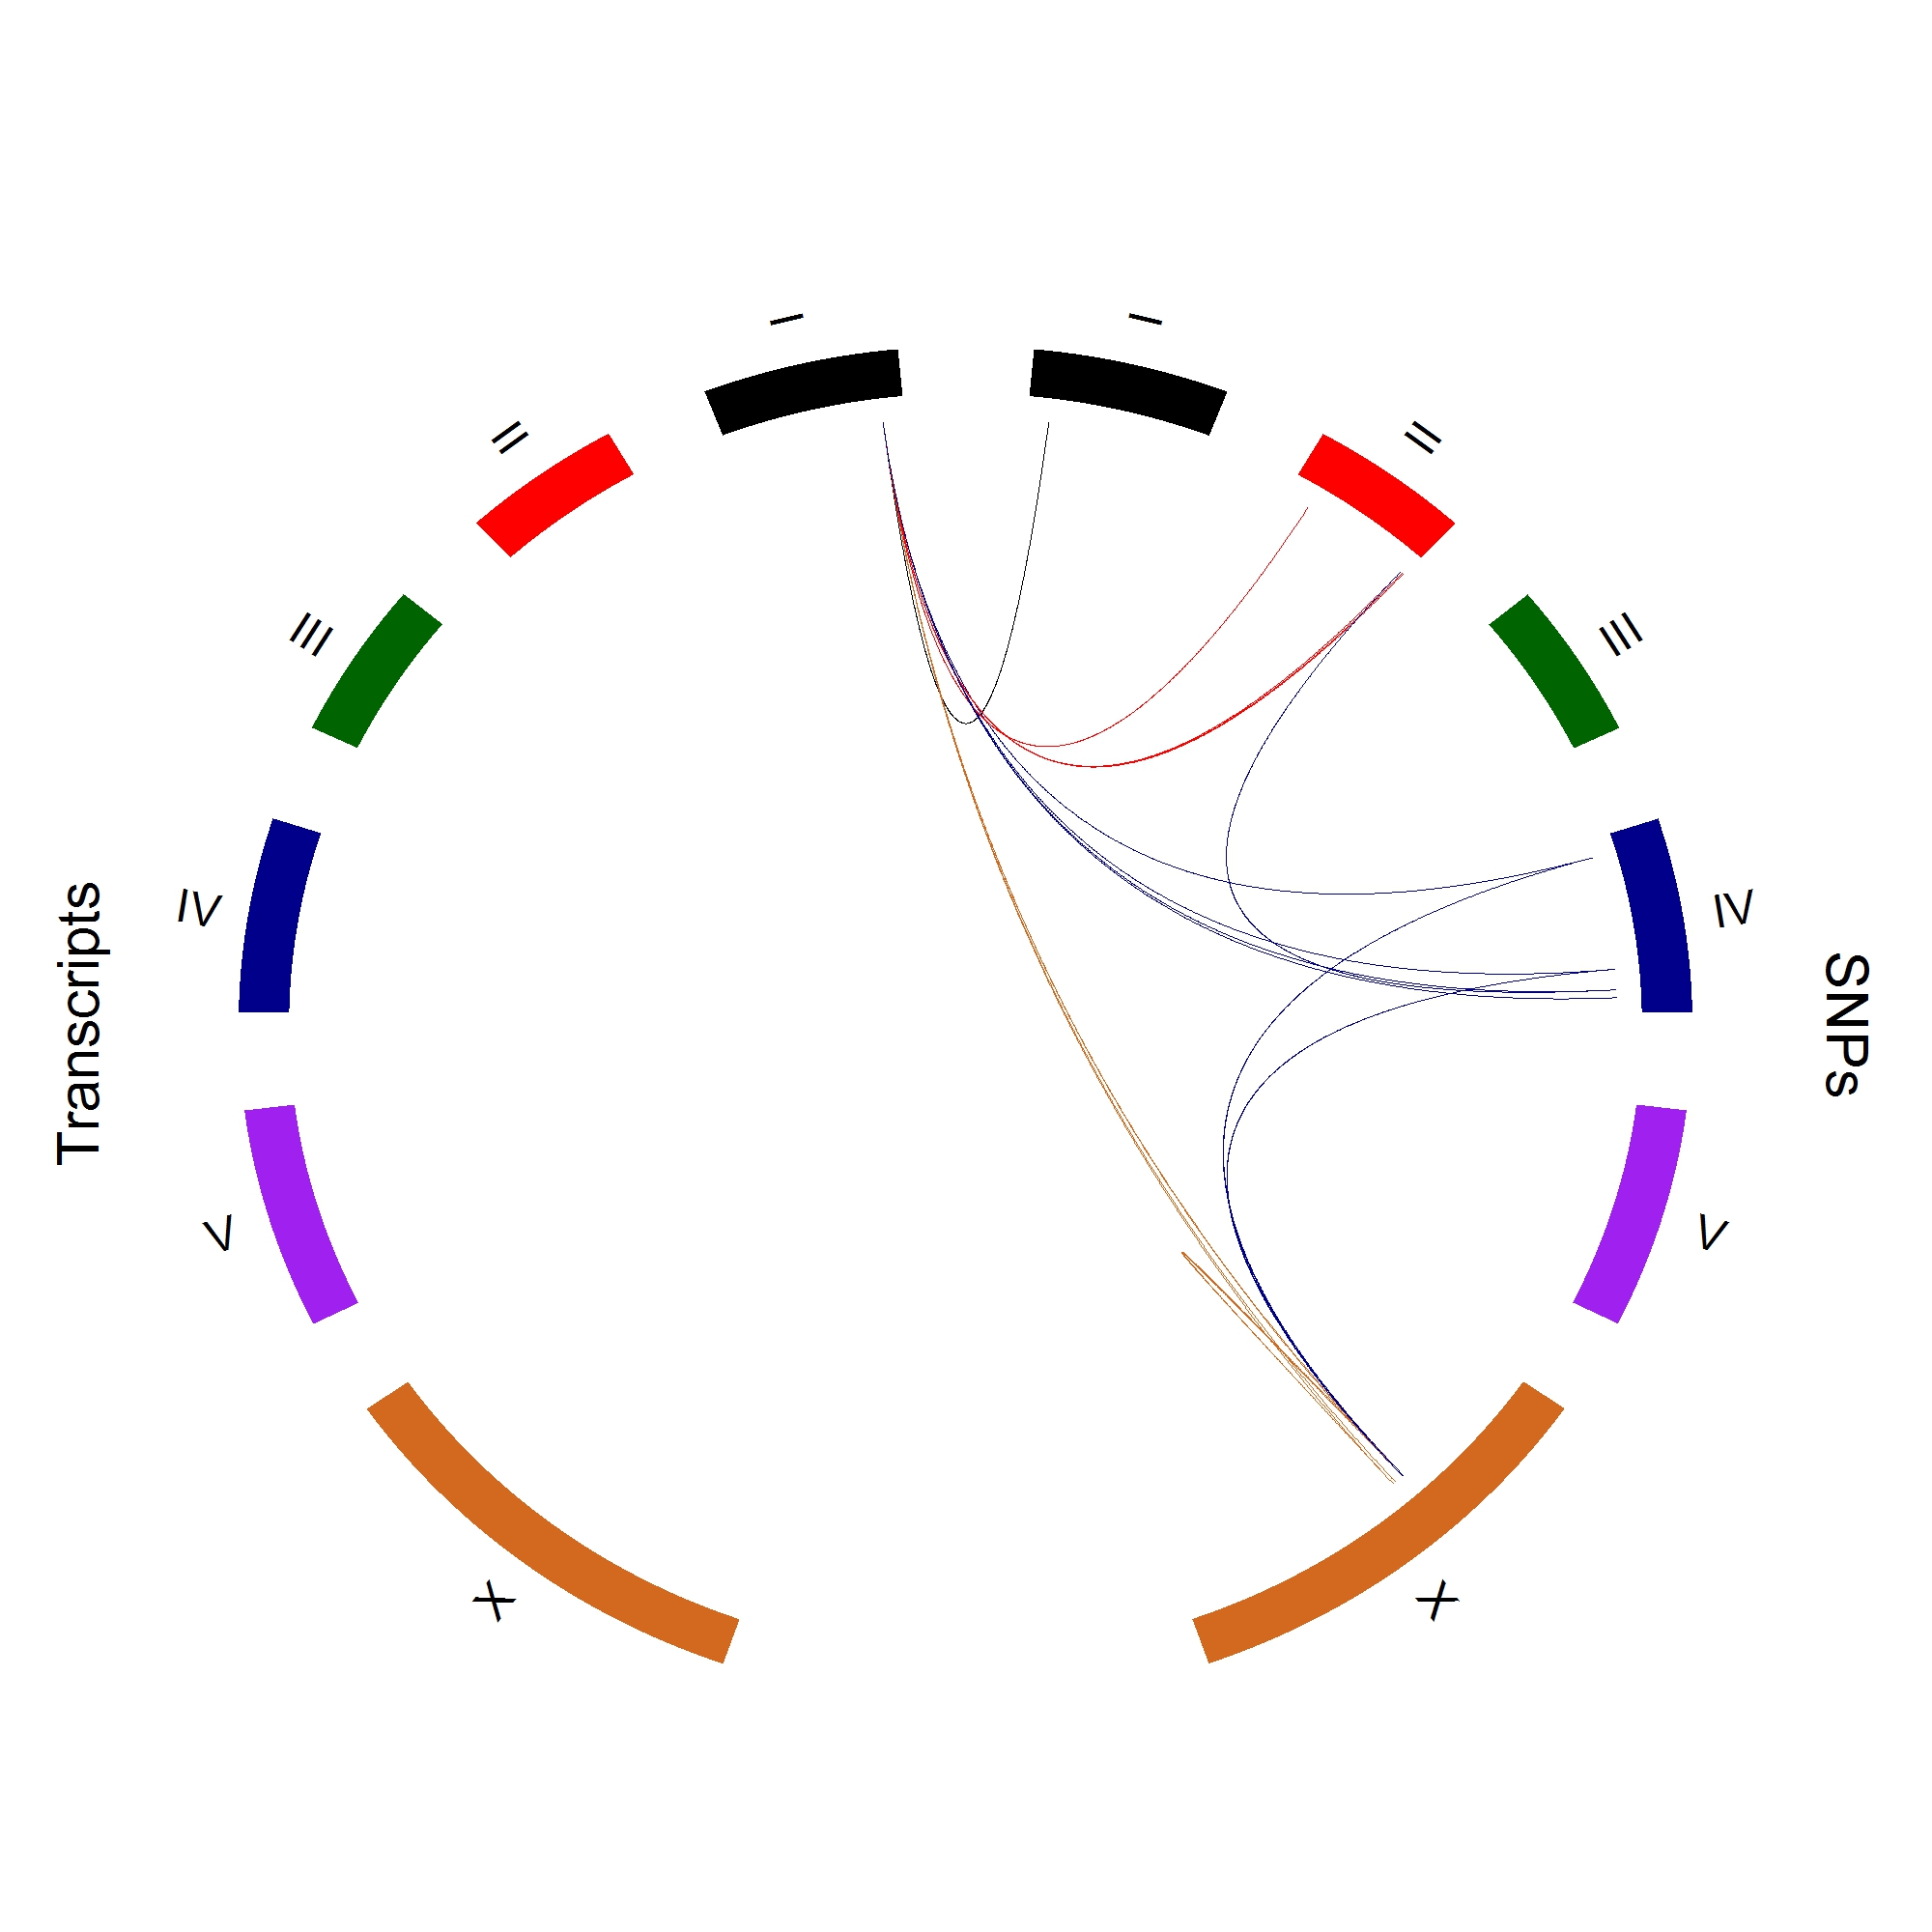
\includegraphics[width=250px,height=250px]{images/iForm_Network_Chr1} 

}

\caption{SNP Picture}\label{fig:ChromosomePic}
\end{figure}

iFORM provides the estimates of each effect (either main effect or
interaction effect), standard errors of each estimate and the
significance tests of each effect. As an example, \ref{tab:OutputTable}
gives the result of how gene transcript A\_12\_P103290 can be predicted
by its eQTLs and their interactions. It can be seen that the final
predictive model (adjusted \(R^2 = 0.896\)) contains 14 markers which
exert their main effects and/or interaction effects on the transcript.
Of the 14 final markers, a half shows significant main effects (p
\textless{} 0.05), with several (i.e., X\_14636404, X4\_15568674,
X4\_15632637 and X\_14542103) explaining about 5\% heritability (defined
as a proportion of genetic variance due to a predictor over the total
phenotypic variance). Of these final markers, we identified eight
significant epistatic interactions. Each epistasis accounts for 4.6 --
5.5\% heritability \ref{tab:OutputTable}.

\begin{table}
\caption{\label{tab:OutputTable}iFORM         Single Marker Analysis}

\centering
\begin{tabular}[t]{lrrrr}
\toprule
eQTL & Effect & SE & p.value & Heritability...\\
\midrule
X1\_2068168 (cis-eQTL) & -0.197 & 0.035 & 0.000 & 0.060\\
X2\_13516256 & -0.069 & 0.039 & 0.080 & 0.007\\
X2\_13813025 & -0.023 & 0.052 & 0.665 & 0.001\\
X2\_13694563 & 0.074 & 0.062 & 0.238 & 0.008\\
X2\_2482896 & 0.064 & 0.027 & 0.017 & 0.006\\
\addlinespace
X\_15500580 & 0.073 & 0.064 & 0.253 & 0.008\\
X\_14636404 & -1.768 & 0.092 & 0.000 & 4.794\\
X4\_16403215 & 0.028 & 0.040 & 0.489 & 0.001\\
X4\_15568674 & -1.972 & 0.134 & 0.000 & 5.964\\
X4\_1873297 & 0.044 & 0.026 & 0.086 & 0.003\\
\addlinespace
X4\_15632637 & 1.960 & 0.143 & 0.000 & 5.892\\
X4\_13532205 & 0.064 & 0.028 & 0.024 & 0.006\\
X\_15820520 & -0.014 & 0.055 & 0.796 & 0.000\\
X\_14542103 & 1.786 & 0.087 & 0.000 & 4.892\\
X2\_13516256.X4\_15632637 & -3.799 & 0.268 & 0.000 & 5.534\\
\addlinespace
X2\_13516256.X4\_15568674 & 3.753 & 0.276 & 0.000 & 5.401\\
X\_15820520.X\_14636404 & -3.771 & 0.172 & 0.000 & 5.453\\
X\_15820520.X\_14542103 & 3.691 & 0.172 & 0.000 & 5.224\\
X\_14636404.X4\_1873297 & -3.534 & 0.163 & 0.000 & 4.789\\
X\_14636404.X4\_13532205 & -3.567 & 0.166 & 0.000 & 4.879\\
\addlinespace
X\_14542103.X4\_1873297 & 3.629 & 0.164 & 0.000 & 5.050\\
X\_14542103.X4\_13532205 & 3.469 & 0.167 & 0.000 & 4.614\\
\bottomrule
\end{tabular}
\centering
\begin{tabular}[t]{rrr}
\toprule
Effect & SE & pvalue\\
\midrule
-0.210 & 0.074 & 0.005\\
-0.138 & 0.075 & 0.068\\
-0.095 & 0.074 & 0.201\\
-0.089 & 0.075 & 0.242\\
-0.057 & 0.076 & 0.453\\
\addlinespace
0.010 & 0.076 & 0.899\\
0.024 & 0.076 & 0.751\\
0.087 & 0.075 & 0.252\\
0.094 & 0.075 & 0.213\\
0.095 & 0.071 & 0.185\\
\addlinespace
0.104 & 0.075 & 0.169\\
0.111 & 0.075 & 0.143\\
0.146 & 0.075 & 0.054\\
0.162 & 0.075 & 0.031\\
NA & NA & NA\\
\addlinespace
NA & NA & NA\\
NA & NA & NA\\
NA & NA & NA\\
NA & NA & NA\\
NA & NA & NA\\
\addlinespace
NA & NA & NA\\
NA & NA & NA\\
\bottomrule
\end{tabular}
\end{table}

It is interesting to note that all predictors jointly contribute to
62.6\% heritability for transcript A\_12\_P103290, of which main effects
account for 26.7\% and epistatic effects account for 35.9\%. It is very
surprising that epistasis contributes to more than a half of
heritability. Of the eight epistatic interactions, only one occurs due
to the interaction between two significant eQTLs, X\_14542103 and
X4\_13532205 \ref{tab:OutputTable}. All the remaining is due to
interactions between one significant eQTL and one non-significant
marker. Some eQTLs, such as X\_14542103 and X\_14636404, produce
epistasis with a greater frequency than others. Despite their
involvement in the final predictive model, some markers were tested to
be insignificant in terms of both main and interaction effects,
suggesting that they regulate a gene transcript in a subtle but
important fashion. In summary, iFORM can not only provide an estimate of
the overall heritability of gene transcript A\_12\_P103290 (i.e., the
sum of individual heritabilities explained by each predictor), but also
chart a detailed picture of how each genetic variant contributes to
transcript variation. In particular, iFORM can characterize epistasis
and its role in trait control, thus equipped with a capacity to retrieve
so-called missing heritabilities (\cite{manolio2009finding}), a
significant issue arising from current genome-wide association studies.

Through analyzing associations between all markers and each transcript
by iFORM, we can identify the difference of cis- and trans-eQTLs for a
particular transcript. For example, of the eQTLs affecting
A\_12\_P103290, we detected that X1\_2068168 is a cis-eQTL, whereas all
others are trans-eQTLs \ref{tab:OutputTable}. We list the number and
distribution of these two types of eQTLs and the pattern of how they
interact with each other to determine gene transcripts \ref{tab:Table5}.
By detecting cis-eQTLs and trans-eQTLs, iFORM detected that genetic
interactions take place mostly between trans-eQTLs.

\begin{table}

\caption{\label{tab:Table5}Distribution of cisQTLs}
\centering
\begin{tabular}[t]{lrr}
\toprule
eQTL.Type & Count & Proportion\\
\midrule
Cis-eQTL & 14 & 0.0024\\
Trans-eQTL & 5509 & 0.9628\\
Cis-eQTL x cis-eQTL & 0 & 0.0000\\
Trans-eQTL x cis-eQTL or cis-eQTL x trans-eQTL & 2 & 0.0003\\
Cis-eQTL x trans-eQTL & 196 & 0.0340\\
\bottomrule
\end{tabular}
\end{table}

\section{Discussion}\label{discussion}

With the recent development of genotyping and sequencing techniques, the
collection of genome-wide genetic and genomic data from any tissue of an
organism has been made much easier and more efficient. Because of this,
genetic studies of complex diseases or traits have developed during the
past decade to a point at which we can draw a complete picture of
genetic architecture for disease or trait formation and progression by
genome-wide association studies (GWAS) (\cite{mackay2009genetics}.
Traditional marginal analysis based on simple regression has been
instrumental for the detection of important genetic variants or
quantitative trait loci in a variety of organisms, but its bottleneck
has emerged quickly due to its limitation in precisely and
comprehensively charting genetic control landscapes. Many GWAS studies
published are bothered by missing heritabilities because of their
incapacity to detect genome-wide epistasis and genotype  environment
interactions (\cite{manolio2009finding}).

Epistasis is a phenomenon by which the influence of a gene on the
phenotype depends critically upon the context provided by other genes
(\cite{cheverud1995epistasis}). It has been increasingly recognized that
epistasis is an important source for trait variation
(\cite{moore2003ubiquitous}; \cite{carlborg2004epistasis};
\cite{cordell2009detecting}), thus inclusion of epistasis would enhance
the prediction accuracy of phenotypic performance and shed more light on
the global genetic architecture of trait control
(\cite{mackay2014epistasis}). However, epistasis is extremely hard to
detect as an interaction term, whose inclusion may complicate the
inference of the predictive model (\cite{carlborg2004epistasis};
\cite{mackay2014epistasis}). Thanks to recent progresses in
high-dimensional data modeling, we have been able to implement several
cutting-edge statistical models for systematical detection and
characterization of genome-wide epistasis.

\cite{hao2014interaction} proposed a new high-dimensional model, iFORM,
that can tackle an issue of interaction selection simultaneously from a
large pool of continuous predictors. This model is based on
forward-selection-based procedures, characteristic of computational
feasibility and efficiency. The authors further proved that the
detection of interactions by iFORM is consistent, even if the dimension
increases exponentially for a sample size. As one of the first attempts
to introduce high-dimensional models into genetic studies, we modified
iFORM to accommodate to the discrete nature of molecular markers. Our
simulation studies indicate that iFORM can provide reasonably accurate
and precise estimates of genetic main effect and interaction effects.
Also, it shows greater power to detect significant genes and their
interactions which may not be detected by traditional single marker
analysis.

We applied iFORM to re-analyze gene expression data in an eQTL mapping
study (\cite{rockman2010selection}). While our results confirmed those
by the traditional approach, the new model provides some new findings
including new eQTLs and epistasis, thus allowing a complete set of
genetic variants to be characterized. As an important tool to understand
the genetic mechanisms underlying both complex traits and diseases, eQTL
mapping has been widely used to identify key regulatory pathways toward
endophenotype and end-point phenotypes (\cite{schadt2005integrative};
\cite{emilsson2008genetics}; \cite{cookson2009mapping};
\cite{pickrell2010understanding}; \cite{nica2013expression}). A typical
eQTL study may not only include a large number of molecular markers as
like in a GWAS, but also record tens of thousands of gene transcripts
throughout the entire genome. Our current version of iFORM can only take
into account one gene transcript as a response at a time, thus having a
limitation to model the correlation and dependence among different
genes. It is our next step to formulate a multivariate multiple
regression model by which to test how an individual predictor, main
effect or epistatic effect, pleiotropically affects correlated
expression profiles of different genes.

Given the complexity of biological phenomena, pair-wise epistasis may be
insufficient to explain phenotypic variation.
\cite{imielinski2008exploiting} argued that high-order interactions
among more than two genes may provide a key pathway toward complex
traits. Three-way interactions have been detected in trait control
(\cite{mcmullen1998quantitative}; \cite{stich2007power}). A model for
modeling three-way interactions has been developed in a case-control
GWAS design (\cite{wang2010general}) and a genetic mapping setting
(\cite{pang2013statistical}). It is crucial to extend iFORM to map main
effect, two-way epistasis and three-way epistasis in an eQTL mapping
study although no substantial change is needed in the computational
algorithm, except for an enlarged test set and extra computing time. Our
work is based on a backcross population in which there are only two
genotypes at a locus. The backcross population can facilitate our
estimation and test of genetic effects owing to a smaller number of
parameters at each locus or locus pair, but its utility is very limited
in the F2 design of model systems and natural populations of outcrossing
species such as humans. A more general model of iFORM should consider
three genotypes at each locus, which provides estimates of additive and
dominant effects at each locus and four types of epistasis, i.e.,
additive x additive, additive x dominant, dominant x additive and
dominant x dominant, between each pair of loci
(\cite{kempthorne1968correlation}). Each of these epistatic types may
affect a phenotype through a different pathway.

With continuous falling of sequencing price, we will have desirable
opportunities to study the dynamic behavior and pattern of gene
expression profiles across time and space scales
(\cite{vinuela2010genome}; \cite{ackermann2013impact}). Many previous
studies suggest that gene expression during cell and organ development
may follow a particular form, which can be quantified by mathematical
equations (\cite{kim2010wavelet}). For example, abundance of gene
expression may change periodically in human's brain during circadian
clock. Many researchers used Fourier's series approximation to model the
periodic changes of gene expression by estimating the period and
amplitude of the cycles (\cite{li2013using}). By integrating Fourier
series into iFORM, we will be able to map dynamic eQTLs for gene
expression and make a quantitative prediction of temporal and spatial
patterns of genetic control by eQTLs.

\hypertarget{highorder}{\chapter{High-order Epistatic
Networks}\label{highorder}}

\section{Motivation}\label{motivation-1}

Quantitative traits are very difficult to study because these traits are
controlled by many genes that interact in a complicated way
(\cite{nelson2013century}; \cite{mackay2014epistasis}). Genome-wide
mapping and association studies increasingly available due to
next-generation high-throughput genotyping techniques have proven to be
useful for characterizing gene-gene interactions, coined epistasis, that
contribute to phenotypic variation (\cite{cordell2009detecting};
\cite{van2011travelling}; \cite{wei2014detecting}). Powerful statistical
methods have been developed to analyze all possible markers
simultaneously, from which to search for a complete set of epistasis for
quantitative traits (\cite{li2014fast}; \cite{gosik2016iform}). The
joint analysis of all markers is particularly needed to chart an overall
picture of genetic interactions, in comparison with computationally less
expensive marginal analysis.

Epistasis reported in the current literature is mostly due to
interactions between two genes. However, a growing body of evidence
shows that genetic interactions involving more than two loci play a
pivotal role in regulating the genetic variation of traits
(\cite{wang2010general}; \cite{dowell2010genotype};
\cite{pang2013statistical}; \cite{taylor2014genetic}). For example, in a
mapping population deriving from crossing two chicken lines, three-locus
interactions were detected to determine body weight
(\cite{pettersson2011replication}). A mapping study established by two
yeast strains identified genetic interactions involving five or more
loci for colony morphology (\cite{taylor2014genetic}). Other studies
have demonstrated that high-order epistasis is of critical importance in
regulating metabolic networks in yeast (\cite{weinreich2013should}) and
Escherichia coli and Saccharomyces cerevisiae
(\cite{imielinski2008exploiting}; \cite{he2010prevalent}), whereas
lower-order (pairwise) epistasis may be insufficient to explain
metabolic variation for these organisms.

The theoretical models of high-order epistasis have well been
established by mathematical biologists (\cite{hansen2001epistasis};
\cite{beerenwinkel2007analysis}). These models provided a foundation to
interpret high-order epistasis from a biological standpoint. A few
statistical models have been derived to estimate and test high-order
epistasis in case-control designs (\cite{wang2015bayesian}) and
population-based mapping settings (\cite{pang2013statistical}).
\cite{wang2015bayesian} developed a Bayesian version of detecting
high-order interactions for both continuous and discrete phenotypes.
However, these models were based on a marginal analysis, thus less
powerful to illustrate a global view of genetic control mechanisms due
to high-order epistasis.

In this article, we deploy a variable selection procedure within a
genetic mapping or association setting to characterize the genetic
architecture of complex traits composed of main effects of individual
genes, pairwise epistasis between two genes, and three-way epistasis
among three genes. The model was built on greedy interaction screening
forward selection developed under the marginality principle (named
iFORM) by \cite{hao2014interaction}. These approaches, proved to possess
sure screening property for ultrahigh-dimensional modeling, have been
implemented to model the genetic architecture of main effects and
pairwise epistasis due to eQTLs for gene transcripts
(\cite{gosik2016iform}). Here, we extend the implementation of iFORM to
systematically capture three-way interactions that are expressed among
all possible markers studied. To show the statistical power of the
extended model, we performed computer simulation studies. The model was
further validated through analyzing a real data of genetic mapping for
shoot growth in a woody plant, mei (Prunus mume). The model should be
used in any other mapping or association studies of quantitative traits.

\section{Methods}\label{methods-1}

\subsection{Mapping and association
studies}\label{mapping-and-association-studies}

Genetic mapping and association studies are two types of designs used to
dissect quantitative traits. The former is based on a controlled cross
derived from distinct parents, whereas the latter samples different
genotypes from a pool of accessions or a natural population. In both
types of design, a set of individuals are sampled to be phenotyped for
quantitative traits of interest and genotyped by molecular markers
distributed throughout the entire genome. For a particular genetic
experiment, the number of markers is much larger than that of samples,
thus, it is impossible to estimate the genetic effects of all markers
simultaneously using traditional regression models. This issue becomes
much intractable when we aim to estimate genetic interactions of
different orders. To tackle the issue of the number of predictors
\textgreater{}\textgreater{} the number of samples, several variable
selection approaches have been implemented in association studies. One
approach is forward selection which was shown to be robust for
estimating pairwise interactions of predictors
(\cite{hao2014interaction}). With sure screening properties and
controlling for false positives, this approach, named iFORM, performs
very well in capturing important information in explaining the response
variable. On top of these nice theoretical properties it is
computationally efficient by using ordinary least squares calculations
and only requiring a predetermined set up steps. Here, we extended the
iForm procedure to include HGI's to capture more relevant information.
In the following sections, the notation and model set-up will be
introduced. After this theoretical properties will be explored. Finally
simulated and real data analysis will be conducted to help confirm the
theoretical properties and show the feasibility of using the model for
screening across whole genomes to more precisely explain phenotypes of
interest.

\subsection{Epistatic model}\label{epistatic-model}

Consider a linear model that underlies the true genotype-phenotype
relationship. Assume that the phenotype, as the response of the model,
is controlled by a set of p SNPs that act singly and/or interact with
each other. These main and interaction effects of markers, i.e., the
predictors of the model, need to be estimated. Let
\(\mathbf{Y}=(y_1,\dots, y_n)^T\) denote the phenotypic value of n
samples from a mapping or association population. When considering
pairwise and three-way interactions, the linear model is expressed as

\begin{equation}
\mathbf{Y}=\alpha + X^T\beta + Z^T\gamma + W^T\eta + \epsilon
\label{eq:lin-mod}
\end{equation}

where \(X=(X_1,\dots,X_p)^T\) is the design matrix that specifies the
genetic effects of each marker
\(\beta=(\beta_1,\dots,\beta_p,~ Z=(X_jX_k)^T (1 \le j \le k \le p)\)
is the design matrix that specifies the epistatic effects between two
markers, expressed in
\(\gamma, W=(X_j X_k X_l)^T (1 \le j \le k \le l \le p)\) is the design
matrix that specifies the epistatic effects among three markers,
expressed in \(\eta\), and \(\epsilon ~ N(0,\sigma^2 )\) is the residual
error normally distributed with mean zero and variance \(\sigma^2\). We
denote the index sets for the linear, order-2 and order-3 effects in
equation \eqref{eq:lin-mod}, respectively, as \(P_1={1,2,\dots,p}\)
\(P_2={(j,k):1 \le j \le k \le p}\)
\(P_3={(j,k,l):1 \le j \le k \le l \le p}\) With the significant main,
order-2 interaction and order-3 interaction effect sets being,
\(T_1={j:\beta_j \ne 0,j \in P_1}\)
\(T_2={(j,k):\gamma_{jk} \ne 0,(j,k) \in P_2}\)
\(T_3={(j,k,l):\eta_{jkl} \ne 0,(j,k,l) \in P_3}\)

The true size of \(\mathcal{T}_1\), will be \(p_1\) and similarly for
\(\mathcal{T}_2\) and \(\mathcal{T}_3\) will have sizes \(p_2\) and
\(p_3\) respectively. There will be a total of 3 sets referred to
throughout the procedure, the candidate set \(\mathcal{C}\), the
selection set \(\mathcal{S}\) and the model set, \(\mathcal{M}\). The
candidate set is the set of all possible predictors at a given step in
the selection process. The selection set contains the predictors that
have previously been selected from the candidate set from each iteration
of the procedure. Finally, the model set is the final model that is fit
from the selection set at the end of the procedure. The BIC is used to
determine the optimal cutoff for the final model size.

\subsection{iForm with high-order
epistasis}\label{iform-with-high-order-epistasis}

The iForm procedure is a forward selecting procedure. In traditional
forward selection the procedure starts with the empty set and then
iterates through the entire set of possible predictors in
\(\mathcal{C}\) and selects the best predictor and includes it in S at
the end of each step. The best predictor can be determined in many ways
but usually is defined by the predictor that results in the least amount
of error. For our purposes we use the residual sum of squares. This
continues with selecting the best predictor from C at each step until a
designated stopping criterion is met or until some information criterion
is met. Common information criteria used for selecting predictors to be
in \(\mathcal{M}\) are AIC, BIC, \(R^2\) and Mallow's \(C_p\) statistic.

The iForm procedure for high-order epistatic detection parallels the
forward selection procedure, but C will grow dynamically with the
creation of order-2 and order-3 interaction effects between main effects
that were included from previous iterations of the procedure. There are
three steps to the model selection. The first step is to initialize the
3 sets mentioned above. The sets, \(\mathcal{S}\) and \(\mathcal{M}\)
are set to the empty set while the candidate set, \(\mathcal{C}\), is
first set to \(P_1\), all the main effects. The next step starts the
forward selection procedure selecting predictors from \(\mathcal{C}\).
The selected predictor will be a main effect at the first step. At
subsequent steps, after interaction effects are included, selected
predictors could be either be a main effect, order-two or order-three
interaction effect. The final step involves repeating the second step
until a designated stopping criterion is met. This can be a certain
amount of predictors to be considered in the final model, or it can be
based off of other factors such as the sample size. The designated
stopping criterion will be denoted as d. For our purposes we use d as a
function of the sample size, \(d = n/log_2a(n)\). The procedure will run
up until d iterations, and the optimal model will then be constructed
from the selection set. This is done by an information criterion. Here
we used the Bayesian Information Criterion proposed by
\cite{chen2008extended} denoted as the \(BIC_2\). This was derived by
them to control the false discovery rate in high dimensional model
selections.

\begin{equation}
BIC_2(\hat{M}) = log(\hat{\sigma_M}^2) + n^{-1} |\hat{M}|*(log(n)+2*log(d^{\star}))
\label{eq:bic2}
\end{equation}

Once the selection procedure is done and there are d predictors in the
selection set the BIC is used to determine the cutoff value for the
optimum number of predictors in the model set. Then linear regression is
performed on the model set.

Two guiding principles are used to help dynamically select the main
effects and epistasis effects throughout the procedure. The first is the
marginality principle, which states that an effect will not be removed
from the model once it has been selected. A previous selected effect may
become marginal by the inclusion of subsequent effects. This especially
can be the case when an interaction effect is included. One of the
parent effects may become less significant or even not significant at
all by considering both in the model. The next principle we state as the
heredity principle but has also been referred to in other work as the
hierarchy principle (\cite{bien2013lasso} and \cite{lim2015learning}).
There are two cases of the heredity principle considered. The strong
case would not allow for an order-2 epistasis effect to be included into
the candidate set without both the parent main effects that make up the
interaction are first included in the model. More formally this can be
written as, \(\gamma_{jk} \ne 0\) only if
\(/beta_j ,\beta_k \ne 0 ~\forall~ 1 \le j, k \le p\). Similarly with
order-3 epistasis, you would need to have all order-2 epistatic parent
effects included in the model before including as a candidate predictor.
This would translate to, \(\eta_{jkl} \ne 0\) only if
\(\gamma_{jk},\gamma_{jl},/gamma_{kl} \ne 0~\forall~ 1 \le j,k,l \le p\).
The weak case relaxes the need for all parent effects to be included in
the model before considering the epistatic effects as candidates. Only
one parent effect would be required to be in the model for candidates to
be included. In the scenario with order-2 epistatic effects we would
need, \(\gamma_{jk} \ne 0\) only if
\(\beta_j^2+,\beta_k^2 \ne 0~ \forall~ 1 \le j, k \le p\) and with
order-3 epistatic effects to be considered as a candidate we would need,
\(\eta_{jkl} \ne 0\) only if
\(\gamma_{jk}^2+\beta_l^2 \ne 0~\forall~ 1 \le j, k, l \le p\).

The heredity (hierarchy) principle help reduce the search space by
making the assumption that previously selected main effects would be
involved in the interaction effects. By considering this principle it
substantially reduces the search space making this feasible for
ultra-high dimensional situations. Even larger than ram datasets can be
used with efficient memory mapping of the dataset while running the
procedure. The weak version of the heredity principle for three-way
interactions states that at least one of the main effects needs to be
selected into the model to consider an interaction effect that contains
that predictor. Considering a moderately high set of predictors say p =
5000, if trying to include all order-2 interactions upfront, will make
the candidate set be as high as 12,498,000. This alone could exceed most
ram requirements of standard computers. This is before even stepping up
to order-3 interactions. The weak heredity principle would decrease the
candidate set substantially. Assuming a sample size of \(n = 200\),
would give a cut off of \(n/log_{2}(n) = 200/log_{2}(200) = 26\) steps
in the procedure. The 5000 original predictors plus up to 5000 epistatic
predictors included in the candidate set at each step in the procedure
would give a maximum of approximately 135,000 candidate predictors. This
would give a maximum of approximately 135,000 candidate predictors. This
gives a 100 fold decrease in the candidate set. This could substantially
make ultra-high dimensional analysis more feasible and also speed it up
in the process. This is the weak case. If considering the strong case
the decrease in candidate space is even more apparent. Aside from the
efficiency by lowering the search space of the candidate set, the
heredity principle is usually taken into account by researchers when
selecting models involving the consideration for interaction effects.

\subsection{Theoretical Properties}\label{theoretical-properties}

The theoretical properties of the iForm procedure with high-order
epistasis follow closely with the forward selection procedure.
\cite{hao2014interaction} summarize forward selection nicely as follows.
At each step, the response is regressed on the most correlated
covariate, and the residual is calculated and used as the new response
in next step. After the most correlated covariate (say, \(X_1\)) is
selected, all other covariates are regressed on \(X_1\), and then the
covariates are substituted by the corresponding normalized residuals,
which are used as the new covariates in next step. By viewing forward
selection in this sense the computational complexity of the procedure
depends upon the size of the candidate set. The candidate set in the
iForm's case does grow dynamically at each step, by at most the number
of predictors currently selected in C for each step. If we denote the
current size of the candidate set as m then each iteration of the
procedure grows with complexity of O(nm), where n is the sample size.
Leaving the selection unrestricted we would not be able to fit more than
n predictors for a linear model and therefore n would be the most main
effects that would be able to be selected. Considering the weakest form
of the heredity principle at the current iteration there would be at
most \(p + (n(n-1)(n-2))/6\) predictors in the candidate set. This would
make the total complexity of the selection procedure to be
\(nO(n(p+n(n-1)(n-2))) = O(n^3 p+n^5)\). This makes the total complexity
grow linearly as p grows.

The theoretical properties of the iForm procedure show sure screening
properties (\cite{fan2008sure}). By this we mean that all the import
predictors, whether that is a main effect or epistatic effect will be
selected with probability tending to 1. This is important to capture as
much of the signal as possible through all the noise that comes with
\(p >> n\) or ultra-high dimensional situations. It is also important
not to `over-fit' the model with unnecessary predictors that actually
explain more noise in the data that the model is being fitted on than
the actual signal you would like to pick up on.

To show the property from above the following conditions would need to
be met for regulatory purposes. \cite{hao2014interaction} showed how
under these conditions sure screening properties for interaction models
like FS2 and iForm are satisfied. This also applies to order-3
interaction models like FS3 and iForm with higher order epistasis, like
we do with the high-order epistasis model. The following assumptions
need to be met for these conditions. The first is that the
\(X=(X_1,\dots,X_p)^T\) are jointly and marginally normal with
independent normally distributed error. Next we would need the
eigenvalues of the covariance matrix to be positive and bounded by two
constants \(0 < \tau_min < 1 < \tau_{max} < \infty\), such that
\(\sqrt{\tau}_min < \lambda_min (\Sigma)≤\lambda_max (\Sigma)< \sqrt{\tau}_max/4\).
Also, the genetic effects, \(\beta\) need a certain level of signal
strength. This we would assume to be \(|(|\beta|)| ≤ C_\beta\) for some
positive constant \(C_\beta\) and
\(\beta_min ≥ \nu\beta \eta^{-\xi_min}\),with \(\beta_min=mina(\beta)\).
Lastly, there needs to be a certain level of sparsity to the number of
important effects. Denoting the total number of important effects as
\(d_0\), and positive constants \(\xi,\xi_0\) and \(\nu\) we would need
\(log(p) ≤ \nu n^\xi,d_0 ≤ \nu n^(\xi_0)\) and
\(\xi+6\xi_0+12\xi_min \lt \frac{1}{2}\). The conditions stated are
accepted standards in the literature when studying ultra-high
dimensional situations. (\cite{hao2014interaction} , \cite{fan2008sure};
\cite{sun2013genome}).

\section{Application}\label{application-1}

\subsection{Simulation Studies}\label{simulation-studies}

To study the numeric properties of the selection procedure, simulation
studies were conducted. Data was generated using R 3.1. The \(X_i\)'s
were all independently and identically distributed realizations
generated from Binomial(0.5) and the true effects for both the main and
epistatic effects were included following different heredity scenarios.
The phenotype was generated from the linear model setup described
previously. To capture relevant data structures, there were several
different scenarios considered. For each scenario 50 predictors were
generated with a sample size of 300 observations. The data was split
into training and a testing set to study both the fitted properties of
the model as well as the generalizability of the model. There were a
variety of metrics obtained to assess the suitability of each model
utilized in the simulations. The first metrics that were taken into
account were the rates for the true positives, false positives, true
negatives and false negatives. Since we have a variety of levels to each
of the models each of the rates were evaluated for the different
hierarchical levels. Some of the models only have main effects and/or
two-way interactions, therefore the rates were only given for the area
applicable to model and the rest were reported as NA. The
generalizability of the models was also assessed by withholding 100
random observations as a test set. All the data was generated from the
same scenario and then 100 of the observations were randomly selected
and stored for out of sample measures. The data was generated from the
given scenario and randomly split before assessing the models. The exact
same training and testing sets were used to fit and assess each of the
models in order to make as fair of a comparison as possible. Each
scenario was replicated 100 times and measures were averaged over all
replicates. The two measures assessed were mean square error and the
coefficient of determination. The analogous in-sample measures were also
calculated for comparison. The models being compared in the simulation
studies are Forward Selection, Forward Selection with all order-2
interactions (FS2), Forward Selection with all order-2 interactions
(FS3), iForm strong heredity order-2, iForm weak heredity order-2, iForm
strong heredity order-3, iForm weak heredity order-3, Glinternet
(\cite{bien2013lasso}), and finally hierNet (\cite{lim2015learning})

Covering a variety of settings the following scenarios were evaluated
and compared.\\
\textbf{Scenario 1:}\\
\(\mathbf{Y}=\beta_1 x_1+\beta_4 x_4+\beta_6 x_6+\beta_7 x_7+\gamma_{1,4} x_1 x_4+\gamma_{1,6} x_1 x_6+\gamma_{1,7} x_1 x_7+\gamma_{6,7} x_6 x_7+\eta_{1,6,7} x_1 x_6 x_7\)
The first is where the data were generated from the interactions of the
model follow a strong heredity (hierarchy) with \(\sigma = 1\). Notice
we have all parent effects of the order-2 epistatic effects and also all
parent effects of the order-3 epistatic effect are also in the model.

\textbf{Scenario 2:}\\
\(\mathbf{Y}=\beta_1 x_1+\beta_4 x_4+\beta_6 x_6+\beta_7 x_7+\gamma_{1,4} x_1 x_4+\gamma_{1,6} x_1 x_6+\gamma_{1,9} x_1 x_9+\gamma_{6,7} x_6 x_7+\eta_{1,6,9} x_1 x_6 x_9\)
The second, the data is generated to have the interactions in follow a
weak heredity (hierarchy) with \(\sigma = 1\). In this scenario the main
effect of \(x_9\) is not included in the model but you can see it is
part of both an order-2 and the order-3 effect.

\textbf{Scenario 3:}\\
\(\mathbf{Y}=\beta_1 x_1+\beta_4 x_4+\beta_6 x_6+\beta_7 x_7+\gamma_{2,3} x_2 x_3+\gamma_{3,8} x_3 x_8+\gamma_{5,8} x_5 x_8+\gamma_{5,9} x_5 x_9+\eta_{3,9,11} x_3 x_9 x_11\)
The third scenario is anti-heredity (hierarchical) where the interaction
effects are only among predictors not present as main effects in the
model. We still have main effects and epistatic effects in the model.
However, the parent effects of the interactions are not the main effects
included in the model.

\textbf{Scenario 4:}\\
\(\mathbf{Y}=\gamma_{1,4} x_1 x_4+\gamma_{1,6} x_1 x_6+\gamma_{1,9} x_1 x_9+\gamma_{6,7} x_6 x_7+\eta_{1,6,9} x_1 x_6 x_9\)
Finally the last scenario only generates data that come from pure
interactions between predictors with no main effects present in the
model used to generate the data.

For the first scenarios where the truth obeys strong heredity where all
of the parent main effects need to be selected before interactions are
selected. The models that appeared to do the best in this simulation
were forward selection on all order-3 interactions included from the
beginning (FS3), iForm order-3 weak heredity and iForm order-3 strong
heredity @ref(tab:Chap3sim1. The FS3 took over a 40 fold increase in
time to run. The other comparison models, glinternet and hierNet seemed
to perform well on the training set but not as well on the testing set.
This would indicate that some overfitting was occurring with those types
of regularization models. The next scenario was when the truth obeys
weak heredity. With the underlying model obeying the weak heredity, the
iForm order-3 strong heredity version dropped off in performance
slightly. However, the FS3 and iForm order-3 remained as top performers
@ref(tab:Chap3sim2. The third scenario assessed was from an underlying
model with an anti-heredity structure. Both main effects and interaction
effects were used in the model to generate the data. However the
interactions included in the model were of combinations of main effects
in the candidate set, that were not in the model. The iForm seems to
drop in performance with this scenario @ref(tab:Chap3sim3. This is to be
expected because it is in direct violation of the underlying assumptions
of the model hierarchy. Even with these violations of the heredity it
still performed reasonably well. Lastly, making the scenario a little
more extreme, the underlying model generating the data was only of
interactions. There were no main effects included in the model. The
results of this scenario are shown in @ref(tab:Chap3sim4. Performance
appeared to drop off for all models explored in the simulation.

\begin{table}

\caption{\label{tab:Chap3sim1}Table 1 Simulation results when the truth obeys strong heredity}
\centering
\begin{tabular}[t]{lrrrrrrrrrrrr}
\toprule
Model & T1.tpr & T1.fpr & T2.tpr & T2.fpr & T3.tpr & T3.fpr & Train.MSE & Train.Rsq & Test.MSE & Test.Rsq & Model.Size & Run.Time\\
\midrule
Forward select & 1 & 0.001 & 0 & 0.000 & 0 & 0 & 3.330 & 0.727 & 3.490 & 0.711 & 4.04 & 0.757\\
Iform weak(2) & 1 & 0.000 & 0 & 0.000 & 0 & 0 & 1.128 & 0.907 & 1.252 & 0.895 & 8.08 & 5.896\\
Iform strong(2) & 1 & 0.000 & 0 & 0.000 & 0 & 0 & 1.102 & 0.909 & 1.198 & 0.900 & 8.00 & 1.557\\
Forward select(2) & 1 & 0.000 & 0 & 0.000 & 0 & 0 & 1.086 & 0.910 & 1.198 & 0.900 & 8.02 & 25.481\\
Forward select(3) & 1 & 0.000 & 0 & 0.000 & 0 & 0 & 0.992 & 0.918 & 1.121 & 0.906 & 8.56 & 471.880\\
\addlinespace
Iform weak(3) & 1 & 0.000 & 0 & 0.000 & 0 & 0 & 1.020 & 0.916 & 1.135 & 0.905 & 9.13 & 11.346\\
Iform strong(3) & 1 & 0.000 & 0 & 0.000 & 0 & 0 & 0.968 & 0.920 & 1.060 & 0.911 & 8.95 & 1.872\\
glinternet & 1 & 0.441 & 1 & 0.018 & 0 & 0 & 1.246 & 0.898 & 1.446 & 0.880 & 29.90 & 208.170\\
hierNet & 1 & 0.303 & 1 & 0.024 & 0 & 0 & 0.906 & 0.925 & 1.421 & 0.882 & 40.99 & 27.521\\
Oracle & NA & NA & NA & NA & NA & NA & 0.953 & 0.921 & 1.050 & 0.912 & 9.00 & NA\\
\bottomrule
\end{tabular}
\end{table}

\begin{table}

\caption{\label{tab:Chap3sim2}Table 2 Simulation results when the truth obeys weak heredity}
\centering
\begin{tabular}[t]{lrrrrrrrrrrrr}
\toprule
Model & T1.tpr & T1.fpr & T2.tpr & T2.fpr & T3.tpr & T3.fpr & Train.MSE & Train.Rsq & Test.MSE & Test.Rsq & Model.Size & Run.Time\\
\midrule
Forward select & 1 & 0.001 & 0 & 0.000 & 0 & 0 & 3.326 & 0.731 & 3.480 & 0.716 & 4.03 & 4.355\\
Iform weak(2) & 1 & 0.000 & 0 & 0.000 & 0 & 0 & 1.119 & 0.910 & 1.200 & 0.901 & 8.07 & 8.342\\
Iform strong(2) & 1 & 0.008 & 0 & 0.000 & 0 & 0 & 1.580 & 0.872 & 1.707 & 0.859 & 7.54 & 2.952\\
Forward select (2) & 1 & 0.000 & 0 & 0.000 & 0 & 0 & 1.083 & 0.912 & 1.167 & 0.904 & 8.00 & 38.872\\
Forward select (3) & 1 & 0.000 & 0 & 0.000 & 0 & 0 & 0.979 & 0.921 & 1.089 & 0.910 & 8.58 & 569.980\\
\addlinespace
Iform weak(3) & 1 & 0.000 & 0 & 0.000 & 0 & 0 & 1.003 & 0.919 & 1.079 & 0.911 & 9.03 & 13.054\\
Iform strong (3) & 1 & 0.008 & 0 & 0.000 & 0 & 0 & 1.578 & 0.872 & 1.705 & 0.859 & 7.58 & 2.787\\
Glinternet & 1 & 0.531 & 1 & 0.020 & 0 & 0 & 0.906 & 0.927 & 1.425 & 0.883 & 33.18 & 29.975\\
hierNet & 1 & 0.343 & 1 & 0.027 & 0 & 0 & 0.856 & 0.931 & 1.412 & 0.884 & 43.43 & 33.302\\
Oracle & NA & NA & NA & NA & NA & NA & 0.940 & 0.924 & 1.034 & 0.915 & 9.00 & NA\\
\bottomrule
\end{tabular}
\end{table}

\begin{table}

\caption{\label{tab:Chap3sim3}Table 3 Simulation results when the truth is anti-heredity}
\centering
\begin{tabular}[t]{lrrrrrrrrrrrr}
\toprule
Model & T1.tpr & T1.fpr & T2.tpr & T2.fpr & T3.tpr & T3.fpr & Train.MSE & Train.Rsq & Test.MSE & Test.Rsq & Model.Size & Run.Time\\
\midrule
Forward select & 1 & 0.000 & 0 & 0.000 & 0 & 0 & 3.284 & 0.729 & 3.510 & 0.714 & 4.02 & 1.005\\
Iform weak (2) & 1 & 0.004 & 0 & 0.000 & 0 & 0 & 3.140 & 0.741 & 3.435 & 0.719 & 4.77 & 7.866\\
Iform strong(2) & 1 & 0.000 & 0 & 0.000 & 0 & 0 & 3.284 & 0.729 & 3.510 & 0.714 & 4.02 & 2.386\\
Forward select (2) & 1 & 0.000 & 0 & 0.000 & 0 & 0 & 1.081 & 0.911 & 1.171 & 0.904 & 8.04 & 29.095\\
Forward select (3) & 1 & 0.000 & 0 & 0.000 & 0 & 0 & 0.989 & 0.918 & 1.095 & 0.910 & 8.59 & 548.620\\
\addlinespace
Iform weak(3) & 1 & 0.003 & 0 & 0.000 & 0 & 0 & 3.155 & 0.739 & 3.448 & 0.719 & 4.57 & 13.216\\
Iform strong(3) & 1 & 0.000 & 0 & 0.000 & 0 & 0 & 3.284 & 0.729 & 3.510 & 0.714 & 4.02 & 2.703\\
glinternet & 1 & 0.710 & 1 & 0.029 & 0 & 0 & 0.844 & 0.931 & 1.578 & 0.871 & 44.59 & 26.564\\
hierNet & 1 & 0.858 & 1 & 0.085 & 0 & 0 & 0.307 & 0.975 & 2.216 & 0.819 & 119.73 & 3.417\\
Oracle & NA & NA & NA & NA & NA & NA & 0.952 & 0.921 & 1.031 & 0.915 & 9.00 & NA\\
\bottomrule
\end{tabular}
\end{table}

\begin{table}

\caption{\label{tab:Chap3sim4}Table 4 Simulation results when the truth is constructed of pure interactions}
\centering
\begin{tabular}[t]{lrrrrrrrrrrrr}
\toprule
Model & T1.tpr & T1.fpr & T2.tpr & T2.fpr & T3.tpr & T3.fpr & Train.MSE & Train.Rsq & Test.MSE & Test.Rsq & Model.Size & Run.Time\\
\midrule
Forward select & NaN & 0.020 & 0 & 0.000 & 0 & 0 & 3.316 & 0.025 & 3.445 & -0.039 & 1.00 & 1.177\\
Iform weak(2) & NaN & 0.028 & 0 & 0.000 & 0 & 0 & 3.007 & 0.115 & 3.181 & 0.040 & 2.27 & 5.840\\
Iform strong(2) & NaN & 0.021 & 0 & 0.000 & 0 & 0 & 3.294 & 0.031 & 3.429 & -0.034 & 1.08 & 2.081\\
Forward select (2) & NaN & 0.000 & 0 & 0.000 & 0 & 0 & 1.117 & 0.669 & 1.170 & 0.644 & 4.01 & 26.396\\
Forward & NA & NA & NA & NA & NA & NA & NA & NA & NA & NA & NA & NA\\
\addlinespace
Select(3) & NaN & 0.000 & 0 & 0.000 & 0 & 0 & 1.005 & 0.703 & 1.081 & 0.671 & 4.62 & 530.360\\
Iform weak(3) & NaN & 0.025 & 0 & 0.000 & 0 & 0 & 3.043 & 0.106 & 3.209 & 0.032 & 1.86 & 9.461\\
Iform strong(3) & NaN & 0.021 & 0 & 0.000 & 0 & 0 & 3.294 & 0.031 & 3.429 & -0.034 & 1.08 & 2.265\\
glinternet & NaN & 0.571 & 1 & 0.017 & 0 & 0 & 1.002 & 0.699 & 1.445 & 0.561 & 27.53 & 145.080\\
hierNet & NaN & 0.853 & 1 & 0.045 & 0 & 0 & 0.672 & 0.802 & 1.758 & 0.467 & 92.52 & 4.491\\
Oracle & NA & NA & NA & NA & NA & NA & 0.968 & 0.713 & 1.022 & 0.689 & 5.00 & NA\\
\bottomrule
\end{tabular}
\end{table}

In the scenarios where the data was assumed to follow some form of a
hierarchical structure for the epistasis effects the iForm procedure for
higher-order epistasis effects appeared to perform the best. Not only
did it result in selecting the correct model, the false positive rate
was also among the lowest. The out of sample error was also among the
lowest between each of the models compared. With the procedure using OLS
calculations, it also performed the fastest out of the models including
epistasis effects. All of the combined show the promise of the iForm
procedure for GWAS type studies. With the other scenarios, the
underlying structure of the data does not follow a typical intuition
about the structure of data in biology.

\subsection{Worked Example}\label{worked-example}

We validated the biological usefulness of the model by analyzing a
mapping data for a woody plant, mei (Prunus mume). Originated in China,
mei has been cultivated for its ornamental flowers for thousands of
years (\cite{sun2013genome}, \cite{sun2014genetic}). Its many desirable
properties, such as cold-hardiness, colors and flavors, are appraised as
a symbol of persistence and beauty in Chinese culture. Recent sequencing
of its genome has made it an ideal model system to study the genetics
and evolution of woody plants (\cite{zhang2013epigenetic}). To improve
the growth rigor and form of mei important to its ornamental value, a
cross was made between two distinct cultivars, Fenban (female parent)
and Kouzi Yudie (male parent), aimed to select superior genotypes from
hybrids. To the end, an F1 mapping population of 190 hybrids was
established and further genotyped for 4,934 SNP markers over eight
linkage groups which correspond to eight chromosomes across the entire
genome.

To test genotypic differences in growth performance, each of these
hybrids was grafted on an established root stock using multiple budding
scions. Next spring, buds on the scions sprouted into shoots. The
lengths and diameters of 10 randomly selected shoots were measured once
every two weeks during an entire growth season from March to October. It
was found that both shoot length and diameter growth was well fitted to
the three-parameter growth equation expressed as

\begin{equation}
g(t) = a/[1+b*exp(-rt)]
\label{eq:growth-curve}
\end{equation}

where \(g(t)\) is the amount of shoot growth at time t, a is the
asymptotic value of growth when time tends to be infinite, b is a
parameter that reflects the amount of growth at time 0, and r is the
relative growth rate. These three parameters determine the overall form
of growth curve jointly, although they function differently. Thus, by
estimating these parameters for individual hybrids using a nonlinear
least squares approach, we can draw the growth curve of each hybrid.
Differences in growth curve among hybrids may be controlled by specific
genes or quantitative trait loci (QTLs). Although tremendous efforts
have been made to map growth QTLs and their epistasis
(\cite{ma2002response};\cite{wu2006functional};
\cite{li2012estimation}), none has characterized the contribution of
high-order epistasis although it has been thought to regulate growth
processes.

By treating the estimates of growth parameters for individual hybrids as
``phenotypic traits,'' we used iFORM to map growth QTLs and QTL-QTL
interactions. Of 4,934 markers, 2,100 are the testcross markers at which
markers are segregating due to only one heterozygous parent and 2,834
are the intercross markers whose segregation results from the
heterozygosity of both parents. For a testcross marker, there is only
one main genetic effect, whereas an intercross marker contains additive
and dominant main effects. Thus, a pair of testcross markers produces
only type of epistasis, but a pair of intercross markers forms four
types of epistasis, additive x additive, additive x dominant, dominant x
additive and dominant x dominant. For two markers with one from the
testcross and the other from the intercross, there are two types of
epistasis, i.e., additive x additive and additive x dominant
(\cite{tong20113funmap}). The number and type of epistasis can be
characterized for any three markers accordingly. Here, the iFORM was
implemented in a way that allows both marker markers to be modeled and
analyzed simultaneously.

To demonstrate the possible importance of high-order epistasis, we
analyze the data by assuming that growth parameters are controlled by
low-order epistasis only and by both low- and high-order epistasis,
respectively. The weak heredity (hierarchical) was used to screen every
SNP and possible interaction of the main effects selected and the rest
of the SNPs left in the candidate set. It was not restricted to the
strong case where both main effects had to be in the model for the
interaction to be considered. For the pairwise epistatic model, this
grew the candidate set to almost 20,000 predictors to choose from. It
turned out that 5 predictors were chosen, i.e., four main additive
effects of markers, AATTC\_nn\_np\_2517, AATTC\_nn\_np\_2815,
CATG\_nn\_np\_3479 and CATG\_nn\_np\_1284 and one epistatic effect due
to markers AATTC\_nn\_np\_2815 and AATTC\_lm\_ll\_3034, for growth
parameter r of shoot length \ref{tab:Chap3Table5}. The main effect of
marker AATTC\_lm\_ll\_3034 was detected to be insignificant. These main
and epistatic effects together explained 32.41\% of the total variance
of parameter r.

\begin{table}

\caption{\label{tab:Chap3Table5}Table 5 The detection of epistasis for the relative growth rate (r) of shoot length in the full-sib family of mei tree by a low-order epistatic model}
\centering
\begin{tabular}[t]{lrrrl}
\toprule
Coefficient & Estimate & SE & T.value & P.value\\
\midrule
(Intercept) & 0.18285 & 0.07613 & 2.402 & 0.0174 *\\
AATTC\_nn\_np\_2517\_a & 0.40013 & 0.06509 & 6.147 & 5.13e-09 ***\\
AATTC\_nn\_np\_2815\_a & 0.15792 & 0.06837 & 2.310 & 0.0221 *\\
CATG\_nn\_np\_3479\_a & 0.23433 & 0.05285 & 4.434 & 1.63e-05 ***\\
CATG\_nn\_np\_1284\_a & 0.22200 & 0.05313 & 4.179 & 4.61e-05 ***\\
AATTC\_nn\_np\_2815\_a×AATTC\_lm\_ll\_3034\_a & 0.45783 & 0.09244 & 4.953 & 1.71e-06 ***\\
\bottomrule
\end{tabular}
\end{table}

When opening up the iForm procedure to the possibility to creating
higher order interactions to be placed into the candidate set, a more
complete picture of the phenotypical variation was revealed. The amount
of predictors included in the final model grew to 12, with one of them
being three-way interactions among markers AATTC\_nn\_np\_2815,
AATTC\_lm\_ll\_3034 and AATTC\_nn\_np\_1615.The adjusted \(R^2\) jumped
up to over 70\% \ref{tab:Chap3Table5}. This astonishing jump in
predictive power is an exemplar case as to the importance of
higher-order interactions in genetic models. Not only did higher-order
interactions become one of the most significant predictors in the model
selected, it also allowed for other order-two interactions and main
effects to be kept in the model that were previously left out. At the
next step of every iteration, the new candidate effect was conditioned
on everything previously selected. With the conditional effect of the
higher-order interaction it enabled for other lost effects to be modeled
as well.

\begin{table}

\caption{\label{tab:Chap3Table6}Table 6 The detection of epistasis for the relative growth rate (r) of shoot length in the full-sib family of mei tree by a high-order epistatic model}
\centering
\begin{tabular}[t]{lrrrl}
\toprule
Coefficient & Estimate & SE & T.value & P.value\\
\midrule
(Intercept) & 0.16859 & 0.05801 & 2.906 & 0.00415 **\\
AATTC\_nn\_np\_2517\_a & 0.27773 & 0.04396 & 6.318 & 2.27e-09 ***\\
AATTC\_nn\_np\_2815\_a & 0.26382 & 0.05295 & 4.983 & 1.54e-06 ***\\
CATG\_nn\_np\_3479\_a & 0.20767 & 0.03467 & 5.990 & 1.23e-08 ***\\
CATG\_nn\_np\_1284\_a & 0.04522 & 0.04265 & 1.060 & 0.29055\\
\addlinespace
AATTC\_nn\_np\_2815\_a×AATTC\_lm\_ll\_3034\_a & 1.82572 & 0.17925 & 10.185 & < 2e-16 ***\\
AATTC\_nn\_np\_2815\_a×AATTC\_hk\_hk\_278\_a & 0.25935 & 0.03888 & 6.671 & 3.48e-10 ***\\
CATG\_lm\_ll\_3153\_a & 0.14877 & 0.03491 & 4.262 & 3.36e-05 ***\\
CATG\_nn\_np\_1284\_a×AATTC\_nn\_np\_554\_a & 0.22994 & 0.05104 & 4.505 & 1.23e-05 ***\\
AATTC\_nn\_np\_2815\_a.AATTC\_lm\_ll\_3034\_a×AATTC\_nn\_np\_1615\_a & -1.51714 & 0.19060 & -7.960 & 2.39e-13 ***\\
\addlinespace
AATTC\_nn\_np\_2815\_a×AATTC\_nn\_np\_929\_a & -0.30805 & 0.05477 & -5.624 & 7.57e-08 ***\\
AATTC\_hk\_hk\_479\_d & 0.16044 & 0.03443 & 4.660 & 6.37e-06 ***\\
AATTC\_nn\_np\_2517\_a×CATG\_hk\_hk\_648\_a & 0.14537 & 0.02840 & 5.118 & 8.33e-07 ***\\
\bottomrule
\end{tabular}
\end{table}

The purpose of the mei genetic project is to study the genetic control
of shoot growth form. Here, we further analyze how three-way
interactions detected by our model affect growth form. Assume that there
are three testcross markers, A (with two alleles A, a), B (with two
alleles B, b), and C (with two alleles C, c), which interact jointly to
affect shoot growth. The three markers form eight genotypes AABBCC,
AABBCc, AABbCC, AABbCc, AaBBCC, AaBBCc, AaBbCC and AaBbCc whose
genotypic means at time t are partitioned into different components,
respectively, expressed as

\begin{figure}

{\centering 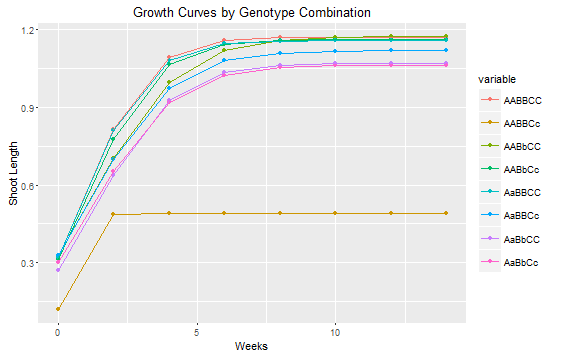
\includegraphics[width=0.8\linewidth]{images/GrowthCurveComparison} 

}

\caption{Growth Curve Comparison}\label{fig:growth-compare}
\end{figure}

\begin{align}
\mu_{111}(t) &= \mu(t) + \alpha_1(t) + \alpha_2(t) + \alpha_3(t) + i_{12}(t) + i_{13}(t) + i_{23}(t) + i_{123}(t)  \notag \\
\mu_{112}(t) &= \mu(t) + \alpha_1(t) + \alpha_2(t) – \alpha_3(t) + i_{12}(t) – i_{13}(t) – i_{23}(t) – i_{123}(t)  \notag \\
\mu_{121}(t) &= \mu(t) + \alpha_1(t) – \alpha_2(t) + \alpha_3(t) – i_{12}(t) + i_{13}(t) – i_{23}(t) – i_{123}(t)  \notag \\
\mu_{122}(t) &= \mu(t) + \alpha_1(t) – \alpha_2(t) – \alpha_3(t) – i_{12}(t) – i_{13}(t) + i_{23}(t) + i_{123}(t)  \notag \\
\mu_{211}(t) &= \mu(t) – \alpha_1(t) + \alpha_2(t) + \alpha_3(t) – i_{12}(t) – i_{13}(t) + i_{23}(t) – i_{123}(t)  \notag \\
\mu_{212}(t) &= \mu(t) – \alpha_1(t) + \alpha_2(t) – \alpha_3(t) – i_{12}(t) + i_{13}(t) – i_{23}(t) + i_{123}(t)  \notag \\
\mu_{221}(t) &= \mu(t) – \alpha_1(t) – \alpha_2(t) + \alpha_3(t) + i_{12}(t) – i_{13}(t) – i_{23}(t) + i_{123}(t)  \notag \\
\mu_{222}(t) &= \mu(t) – \alpha_1(t) – \alpha_2(t) – \alpha_3(t) + i_{12}(t) + i_{13}(t) + i_{23}(t) – i_{123}(t)
\label{eq:genetic-effects}
\end{align}

where \(\mu(t)\) is the population mean at time t; \(\alpha_1(t)\),
\(\alpha_2(t)\), and \(\alpha_3(t)\) are the genetic effects of markers
A, B and C at time t, respectively; \(i_{12}(t)\), \(i_{13}(t)\), and
\(i_{23}(t)\) are the pairwise epistatic effects between markers A and
B, A and C and B and C at time t, respectively; and \(i_{123}(t)\) is
the three-way epistatic effect among three the markers at time t. From
the above equations, we solve the pairwise and three-way epistatic
effects as

\begin{figure}

{\centering 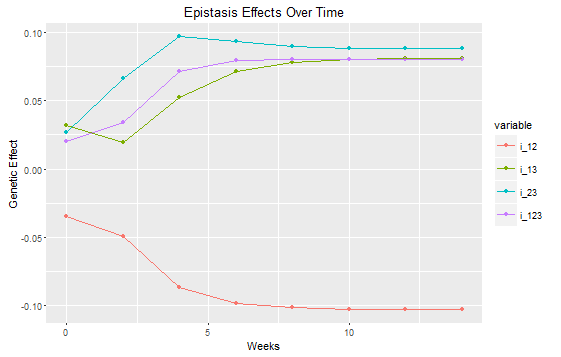
\includegraphics[width=0.8\linewidth]{images/EpistasisComparison} 

}

\caption{Epistasis Comparison}\label{fig:epistasis-compare}
\end{figure}

\begin{align}
i_{12}(t) &=  [(\mu_{111}(t) + \mu_{112}(t) + \mu_{221}(t) + \mu_{222}(t)) – (\mu_{121}(t) + \mu_{122}(t) + \mu_{211}(t) + \mu_{212}(t))] \notag \\
i_{13}(t) &=  [(\mu_{111}(t) + \mu_{121}(t) + \mu_{212}(t) + \mu_{222}(t)) – (\mu_{112}(t) + \mu_{122}(t) + \mu_{211}(t) + \mu_{221}(t))] \notag \\
i_{23}(t) &=  [(\mu_{111}(t) + \mu_{122}(t) + \mu_{211}(t) + \mu_{222}(t)) – (\mu_{112}(t) + \mu_{121}(t) + \mu_{212}(t) + \mu_{221}(t))] \notag \\
i_{123}(t) &=  [(\mu_{111}(t) + \mu_{122}(t) + \mu_{212}(t) + \mu_{122}(t)) – (\mu_{112}(t) + \mu_{121}(t) + \mu_{211}(t) + \mu_{222}(t))]
\label{eq:epi-effects}
\end{align}

Each genotype can draw a growth curve using its growth parameters (a, b,
r) estimated from raw data, from which we can chart the curves of
pairwise and three-way epistatic effects using equation
\eqref{eq:genetic-effects}. Three markers AATTC\_nn\_np\_2815(AA/Aa),
AATTC\_lm\_ll\_3034(BB/Bb) and AATTC\_nn\_np\_1615(CC/Cc) that produce a
significant three-way interaction for parameter x of shoot length
display pronounced differences in growth curve \ref{fig:growth-compare}.
The epistasis of low- and high-order performs differently to affect
growth form, with three-way interactions playing a more remarkable role
than pairwise epistasis \ref{fig:epistasis-compare}.

The figures display the variation between each of the growth curves for
the eight combinations of the three marker genotypes focused on
\ref{fig:growth-compare}. Differences of each of the growth parameters
can be observed when studying the figures. There is clear separation in
the shoot length that is observed at the end of the 16 weeks. This
difference can be visually grouped into four clusters that show the
effect a genotype combination can have on the asymptotic growth
parameter, a. Another noticeable different between the curves displayed
is the rate at which the growth developed. At the earlier weeks of
development you can see some of the genotype combinations grew faster,
manifesting in a steeper slope and other genotypes had shallower slopes.
All of these visually show what was picked up on when modeling the shoot
length growth and the impact of the higher-order interactions between
the genotypes have on such growth. By solving the system of linear
equations in \eqref{eq:epi-effects} we can dissect the epistatic effects
of the genotype combinations. The effects over time are displayed
\ref{fig:epistasis-compare} and in this you can see the non-linear
influence of the interactions between the markers included.

\section{Discussion}\label{discussion-1}

Genetic interactions have been thought to contribute to a significant
portion of genetic variance for quantitative traits of critical
importance to evolutionary biology, agriculture and medicine
(\cite{nelson2013century}; \cite{mackay2014epistasis}). While pairwise
interactions have been a major focus of quantitative genetic studies,
there has been growing evidence that genetic interactions involving
three or more loci play an important role in affecting the phenotypic
differentiation of traits (\cite{wang2010general};
\cite{dowell2010genotype}; \cite{pettersson2011replication};
\cite{pang2013statistical}; \cite{weinreich2013should};
\cite{taylor2014genetic}; \cite{taylor2015higher}). Because of its
complexity due to a network of interactions, the detection of high-order
epistasis is extremely difficult (\cite{mackay2014epistasis}). More
importantly, interpretation of high-order epistasis and its contribution
to overall genetic architecture can be better made by jointly analyzing
all possible low- and high-order interactions among genes. This has
added an extra challenge to statistical modeling and detection of this
important phenomenon. Thanks to the recent development of statistical
models for high-dimensional variable selection, we have reformed a
statistical modeling framework for detecting high-order epistasis by
focusing on three-way interactions.

Our model extends \cite{hao2014interaction} forward selection-based
algorithm iFORM that has proven to be robust and efficient for computing
and detecting two-way interactions between predictors (including
continuous predictors). A favorable property of iFORM is its capacity to
detect interactions even if the dimension of predictors is extremely
high relative to a sample size used. The fundamental assumption used by
iFORM is the heredity principle, i.e., the existence of interactions
between a pair of variables that each has at least weak main effects.
After extending it to characterize three-way interactions, this
assumption can be relaxed for the third variable; i.e., even if there is
no detectable main effect for the third marker, then extended iFORM can
still detect the three-way interaction. This property may explain the
reason why high-order epistatic model outperforms low-order epistatic
model, as demonstrated from the detection of significant genetic
interactions in a real data of a woody plant, mei (Prunus mume). It was
found from a recent study that loci participating in high-order genetic
interactions may not individually have measurable effects
(\cite{bloom2013finding}). As a result, our model can be used as a
general tool to detect genetic interactions of various orders and,
therefore, elucidate the overall picture of genetic architecture by
capturing the so-called missing heritability.

The model was investigated by simulation studies whose result help users
to determine an optimal design of mapping or association studies in
terms of sample size, phenotyping precision and the number of markers.
Its application to P. mume genetic mapping leads to the detection of key
loci and their interactions expressed at the low- and high-order levels
for the growth form of shoots. The curve of three-way epistasis on mei
shoot length growth was observed to increase exponentially during the
first five weeks of shoot sprouting and become stable after five weeks.
Such integration of the model into growth equation shed light on the
developmental mechanisms of growth processes through epistasis, a
question that has evoked a tremendous interest of researchers globally
in the area of evolutionary developmental biology
(\cite{franks2007rapid}, \cite{cartolano2015heterochrony},
\cite{nishino2013network}). We have created an R package that has
implemented the model which adds a function to allow epistasis of any
orders to be searched. The package can be uploaded at
\url{http://statgen.psu.edu/software/} and will be made available
through CRAN (Comprehensive R Archive Network).

\hypertarget{iformfunc}{\chapter{iForm Functional
Mapping}\label{iformfunc}}

\section{Motivation}\label{motivation-2}

As we have seen and also has been noted by several researchers while
conducting biometric analysis (\cite{jinks1982biometrical};
\cite{hill2004ds}; \cite{wu1996detecting}) or molecular dissection
(\cite{mackay2009genetics}, \cite{park2010estimation}) is that
quantatitve traits are very complex and much is still needed to be
learned. The researchers cited note that the traits are most likely
polygenic, including gene-gene interactions and other sources of
interaction effects. (\cite{cheverud1995epistasis};
\cite{moore2003ubiquitous}; \cite{van2010detection};
\cite{mackay2014epistasis}) Higher order interactions of complex traits
are not well studied because of their difficulty to detect in mapping
studies as well. The lack of data should not be construed as proof that
this order of interaction does not exist. (\cite{taylor2015higher}). The
difficulty in detection leads a way for new computational methods to be
developed and approaches to describe how to distinguish such effects. As
noted in chapter \ref{highorder}, new theoretical models of high-order
epistasis have well been established by mathematical biologists
(\cite{hansen2001epistasis}; \cite{beerenwinkel2007analysis}). These
models provided a foundation to interpret high-order epistasis from a
biological standpoint. A few statistical models have been derived to
estimate and test high-order epistasis in case-control designs
(\cite{wang2015bayesian}) and population-based mapping settings
(\cite{pang2013statistical})

Growth and developmental traits are mostly better described by a
functional process (\cite{hernandez2015understanding},
\cite{muraya2017genetic}), it is more biologically meaningful to map
these traits as growth curves (\cite{sun2015mapping}). There have been a
few different approaches that have integrated growth equations into
genetic mapping via the likelihood function, leading to the birth of a
so-called functional mapping models (\cite{ma2002functional};
\cite{wu2006functional}; \cite{li2015dynamic};
\cite{muraya2017genetic}). These style of approaches can allow for the
developmental change of genetic control to be characterized across both
time and as well as space (\cite{he2010mapping};
\cite{li2010functional}). Treating the phenotype as a complex trait it
would be likely it would follow a more functional or dynamic process.
This information could be lost or greatly limited by treating the
response as a single static predictor. Modeling the longitudinal
structures in this fashion, functional mapping has proven to be of great
statistical power in gene identification and the utilization of sparse
phenotypic data (\cite{hou2006framework}). In an attempt to capture all
relevant information and be as parsimonious as possible principles from
biophysical and biochemical processes were considered. The logistic
growth equations are both biologically relevant (\cite{west2001general};
\cite{sun2014model}) and have few parameters that can be mapped to
growth QTLs by estimating these parameters for each genotype and
interactions between genotypes.

There are many approaches for gene mapping with genome-wide association
studies (GWAS) being one of the most popular one, achieving a
considerable success since their first publication in 2005
(\cite{klein2005complement}). Analytical approaches are constantly being
developed to perform GWAS studies. There are a few areas of challenges
in statistical modeling and analysis of genetic data that account for
the complexity of phenotypic information. Generally GWAS studies
associate genetic markers with static, single valued phenotypes. As we
have discussed, most analysis revolve around point wise estimates and do
not always take the entirety of the system during the analysis.
Incorporating selections are starting to become more common but further
work is this area still needs to be explored. Extending the forward
selecting procedure previously state in \ref{highdeqtl} and
\ref{highorder} in order to handle a functional phenotype would be very
beneficial with GWAS level studies. A few challenges do arise while
considering to conduct a genome-wide association study (GWAS) on
interacting traits measured at a sequence of time points. The model
needs to be flexible enough to fit different situations, independence of
the error structure needs to be maintained or accounted for with the
time dependencies and finally computational efficiency needs to be good
enough to fit such complex models. All of these issues combined make it
a difficult exertion to take on but with computational power increasing,
it is becoming more feasible to handle.

In applications like the scenario described where we have a functional
value phenotype and a high dimensional predictor space with dynamically
considering interaction effects it may be too restrictive to suppose
that the effect of all of the predictors is captured by a simple linear
fit. Reframing the regression problem to help code in the longitudinal
data into the structure in a biologically meaningful manner and making
some sparsity assumptions about the number of significant genetic and
epistatic effects that affect the phenotype will help in the development
of such a model to tackle such a task.

\section{Methods}\label{methods-2}

\subsection{Regression by linear combination of basis
functions}\label{regression-by-linear-combination-of-basis-functions}

One common approach to regression problems is to frame the model as a
linear combination of basis functions. In typical multiple regression
the design matrix would be the values of the observed predictors and
these would be used to fit the model, usually with a least squares
approach. The goal then being to fit the expected value of the phenotype
of interest in terms of the values of the predictors. This would result
in a linear model of the form,

\begin{equation}
\mathbf{Y} = \beta_0 + \beta_1 X_1 + \dots + \beta_p X_p + \epsilon
\label{eq:lin-mod}
\end{equation}

This model is nice for a single response but can be too restrictive at
times. With a functional response over time, having a model with more
flexibility could more accurately estimate the phenotype especially when
considering a functional phenotype like a growth model. A fit like the
one mentioned would only restrict growth to be a straight line and that
may not be applicable in real world applications. By treating the
problem as linear combination of basis functions, the general form would
look like,

\begin{equation}
f(x) = \sum_{i=0}^P \theta_i \phi_i(x)
\label{eq:gen-form}
\end{equation}

where the \(\phi\) are the basis functions of the researchers choosing.
Under this format you can choose any function that would fit the need of
the given problem and has relevance to the application area. A common
choice is to use polynomial regression, where \(\phi\) would be the
predictors raised to different degrees in order to invoke a non-linear
relationship into the model. This works well but it comes with some draw
backs. The first being that for each degree consider, it could grow the
predictor set even larger. Instead of just one effect for each predictor
you could have up to the order of the polynomial effects for each
predictor. With the predictor set being at a high dimensional level
already, this may not be something feasible to do. The other area of
concern is that it would give a way for higher correlation between
effects in the model. This would violate the initial assumptions of the
model.

Standard polynomial regression is just one case of using basis functions
in linear regression. There are many transformations that are able to be
performed to invoke nicer properties to the data. The basis functions
that are going to be focused on in this work are orthogonal polynomials.
This would be a special case of polynomial regression that would
alleviate some of the drawbacks mentioned above. Orthogonal polynomials
by definition are orthogonal to each other and therefore would not have
any correlation between predictors when used as basis functions. Also as
an advantage, polynomial regression can be used to make similar types of
interest as other types of multiple regression analysis. It does this
while modeling a non-linear relationship between the phenotype and
genetic markers without having to use complex optimization methods.
Ordinary least squares would still apply in this framework, making it
more computational efficient as well. One specific class of orthogonal
polynomials that will be used are the Legendre polynomials because of
the nice properties they posses.

\subsection{Legendre Polynomials}\label{legendre-polynomials}

\begin{figure}

{\centering 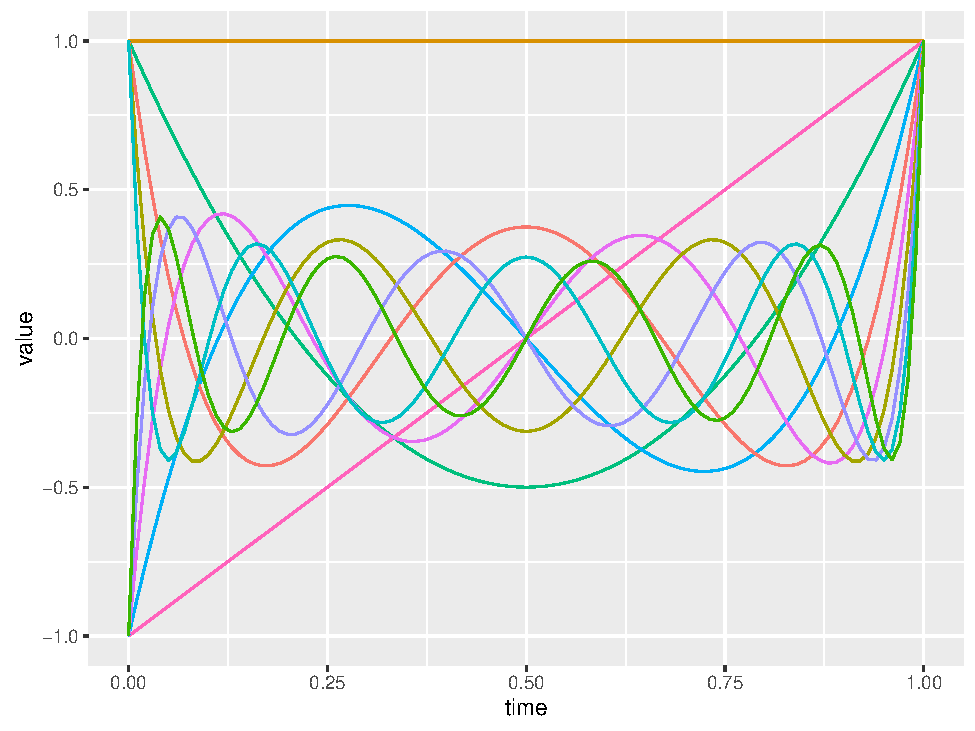
\includegraphics[width=0.8\linewidth]{Defense_files/figure-latex/Legendre-fig-1} 

}

\caption{First 10 Legendre Polynomials}\label{fig:Legendre-fig}
\end{figure}

The definition of the Legendre polynomials are the solutions for \$n =
0, 1, 2, \dots \$ (with the normalization \(P_n(1) = 1\) form a
polynomial sequence of orthogonal polynomials called the Legendre
polynomials. Each Legendre polynomial \(P_n(x)\) is an nth-degree
polynomial. It may be expressed using Rodrigues' formula:

\begin{equation}
P_n(x) = \frac{1}{2^nn!} \frac{d^n}{dx^n}[(x^2-1)^n]
\label{eq:rodrigues-formula}
\end{equation}

An important property of the Legendre polynomials is that they are
orthogonal with respect to the L2-norm on the interval
\(−1 \le x \le 1\):

\begin{equation}
\int_1^{-1} P_m(x)P_n(x)dx = \frac{2}{2+1}\delta_{mn}
\label{eq:orthg-leg}
\end{equation}

\(\delta_{mn}\) denotes the Kronecker delta equal to 1 if m = n and 0
otherwise. These polynomials can be generated by using the following
recursively. Each Legendre polynomial would be the next order n in the
expression below.

\begin{equation}
\begin{split}
P_n(x) & = \frac{1}{2^n}\sum_{k=0}^{n}{{n}\choose{k}}^2(x-1)^{n-k}(x+1)^k \\
& = \sum_{k=0}^{n}{{n}\choose{k}}{{-n-1}\choose{k}}{\left(\frac{1-x}{2}\right)}^k \\
& = 2^{-n}\sum_{k=0}^{n} x^k {{n}\choose{k}}{{\frac{n+k+1}{2}}\choose{k}} \\
\end{split}
\label{eq:leg-eq}
\end{equation}

With the nature of the Legendre orthogonal polynomials, it was
advantageous for both dimension reduction and also handling unevenly
spaced, missing or non-uniform time measurements from different subjects
in the dataset. By seeing which polynomial curve fits the given
phenotype, it removes some of the challenges when fitting the model.
Different orders of the polynomial are tried throughout the procedure to
allow for flexibility in the fitting the genetic variation from the mean
curve for each of the genotypes or epistasis between genotypes
considered in the model.

\subsection{Model}\label{model}

The layout of the underlying model is first fit to an asymptotic growth
model described by a logistic curve of the form,

\[\mu(t) = a/(1 + b * exp(-r*t))\]

It is biologically meaningful to implement a growth equation, like a
logistic curve, to describe growth trajectory \cite{west2001general}.
Here the population is described by a mean growth curve by this growth
equation where a, b and r are growth parameters each provide a
biological interpretation, with a being the asymptotic growth, b being
the initial amount of growth and r being the relative growth rate. Time
varying additive and dominant effects of significant SNPs are modeled by
the Legendre orthogonal polynomial used in quantitative genetic studies,
mentioned above. (\cite{jiang20152higwas}, \cite{olori1999estimating},
\cite{li2010functional}). This representation can be expressed as

\[ \alpha_j(t) = (L_0(t), L_1(t), ... , L_s(t))*(u_{j0}, u_{j1},...,u_{js})^T \]
\[ \beta_j(t) = (L_0(t), L_1(t), ... , L_{s'}(t))*(v_{j0}, v_{j1},...,v_{js'})^T \]

where \(L_0(t), L_1(t), ... , L_s(t)\) and
\(L_0(t), L_1(t), ... , L_{s'}(t)\) are the LOP of orders \(s\) and
\(s'\), respectively; and \(u_{j0}, u_{j1},...,u_{js}\) and
\(v_{j0}, v_{j1},...,v_{js'}\) are the vectors of time-invariant
additive and dominant effects, respectively. Orders \(s\) and \(s'\),
selected from information criteria, for the purposes of this procedure
the Bayesian information criterion (\(BIC_2\)), originally developed by
\cite{chen2008extended} was implemented. A nice feature that comes from
modeling the fit in this manner is that the dimension of response data
is reduced through LOP modeling. (\cite{li2010functional},
\cite{jiang20152higwas}, \cite{li2010functional},
\cite{ahn2010functional}, \cite{das2011dynamic}). Writing the model out
more explicitly we would have,

\begin{equation}
\begin{split}
y(t) = \mu(t) + \sum_{j=1}^{J}\alpha_j(t)\xi_j + \sum_{k=1}^{K}\beta_k(t)\zeta_k \\ 
&+ \sum_{I_1<I_2=1}^{I}\gamma_I^{aa}(t) \xi_{I_1}\xi_{I_2} \\ 
&+ \sum_{I_1<I_2=1}^{I}\gamma_I^{ad}(t) \xi_{I_1}\zeta_{I_2} \\
&+ \sum_{I_1<I_2=1}^{I} \gamma_I^{da}(t) \zeta_{I_1}\xi_{I_2} \\
&+ \sum_{I_1<I_2=1}^{I} \gamma_I^{dd}(t)\zeta_{I_1}\zeta_{I_2} \\ 
&+ \epsilon(t)
\end{split}
\label{eq:epi-legendre}
\end{equation}

\subsection{Incorporating with the iForm
Procedure}\label{incorporating-with-the-iform-procedure}

We start off with the underlying assumption that our final model will be
of the following form.

\[
\begin{equation}
\begin{split}
y(t) = \mu(t) + \sum_{j=1}^{J}\alpha_j(t)\xi_j + \sum_{k=1}^{K}\beta_k(t)\zeta_k + \sum_{I_1 \lt I_2=1}^{I}\gamma_I^{aa}(t) \xi_{I_1}\xi_{I_2} \\ 
+ \sum_{I_1 \lt I_2=1}^{I}\gamma_I^{ad}(t) \xi_{I_1}\zeta_{I_2} + \sum_{I_1 \lt I_2=1}^{I} \gamma_I^{da}(t) \zeta_{I_1}\xi_{I_2} + \sum_{I_1 \lt I_2=1}^{I} \gamma_I^{dd}(t)\zeta_{I_1}\zeta_{I_2} + \epsilon(t)
\end{split}
\end{equation}
\] where,

\[\mu(t)=\frac{a}{(1+b*exp\{-r*t\})}\]
\[ \alpha_j(t) = (L_0(t), L_1(t), ... , L_s(t))*(u_{j0}, u_{j1},...,u_{js})^T \]
\[ \beta_j(t) = (L_0(t), L_1(t), ... , L_{s'}(t))*(v_{j0}, v_{j1},...,v_{js'})^T \]

An outline of the selection procedure used following the model described
is as follows. At first the mean growth curve is estimated for the
presented data following the logistic growth curve. This could be
adjusted depending on the functional process the researcher is studying.
Once the mean curve is fit the selection procedure is initialized in a
similar fashion as mentioned in previous chapters @ref\{highdeqtl\}.
Both the solution set is assigned to the empty set, \(S_0=\emptyset\)
and the model set is set to just the fitted growth curve as an
effect.\(M_0=\mu(t)\). The candidate set begins with containing all main
effects for the additive and dominant effects of each SNP. The selection
procedure then begins and each SNP is assessed and the best fitting
candidate is then placed in the selection set. While assessing each
candidate SNP, an additional search is performed for the best fitting
polynomial fit up to a pre-specified order that is determined at the
beginning of the procedure. The orthogonal polynomials are used to
assist in fitting the genetic effects for each marker or epistatic
interaction between the markers. This would allow the genetic effect
some flexibility over time and give a more representative fit. This
could also be used with other functional models or other types of
non-linear functions that characterizes the biological systems being
evaluated. We are treating the polynomials as a basis function for the
regression problem and therefore the residual sum of squares is
calculated similar to generalized least squares but replacing the design
matrix with the necessary basis functions. This continues until a
designated stopping value is reached. The \(BIC_2\) is then used to find
the optimal fit given the selection set produced by the procedure. The
following graphics show how the process works at each step

\begin{itemize}
\tightlist
\item
  Step 1: (Growth Curve) Fit the mean growth curve to the response data
  and use as an intercept term.\\
\item
  Step 2: (Initialization) Set \(\mathcal{S}^{(0)} = \emptyset\),
  \(\mathcal{M}_0 = \mu(t)\) and \(\mathcal{C}_0 = \mathcal{P_1}\)
\item
  Step 3: (Selection) In the kth step with given
  \(\mathcal{S}^{(k-1)}\), \(\mathcal{C}^{k−1}\) and
  \(\mathcal{M}^{k−1}\), forward regression is used to select one more
  predictor from \(\mathcal{C}^{k−1}/ \mathcal{S}^{k−1}\) into the model
  while checking for different degrees of the legendre polynomial used
  as a basis for the genetic effect. We add the selected one into
  \(\mathcal{S}^{k−1}\) to get \(\mathcal{S}^k\). We also update
  \(\mathcal{C}^k\) and \(\mathcal{M}^k\) if the newly selected
  predictor is a main effect. Otherwise,
  \(\mathcal{C}^k = \mathcal{C}^{k−1}\) and
  \(\mathcal{M}^k = \mathcal{M}^{k−1}\)
\item
  Step 4: (Solution Path). Iterating Step 2, for D times, which leads to
  a total of D nested candidate models. We then collect those models by
  a solution path \(\mathbb{S}=\{\mathcal{S}^{(k)}: 1 \le k \le D\}\)
\end{itemize}

\begin{figure}

{\centering 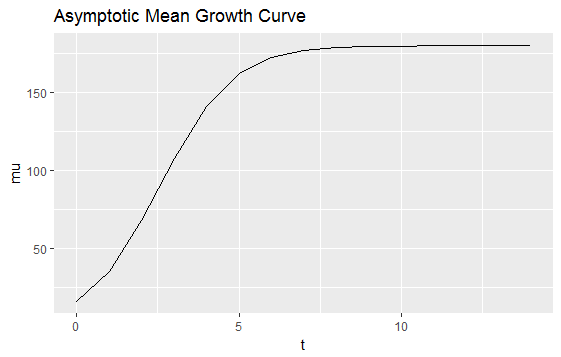
\includegraphics[width=0.8\linewidth]{images/GrowthCurveExample} 

}

\caption{Intial Growth Curve Fit}\label{fig:growth-example}
\end{figure}

\begin{figure}

{\centering 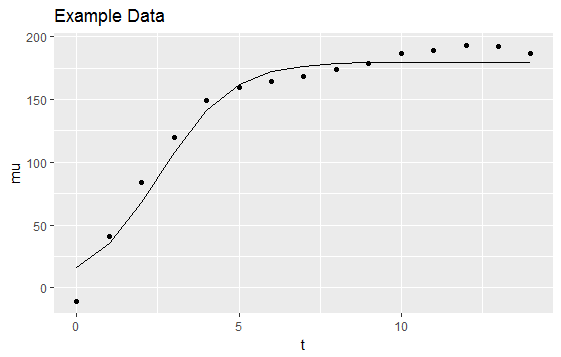
\includegraphics[width=0.8\linewidth]{images/ExampleDataGrowthCurve} 

}

\caption{Growth Cruve with Example Data}\label{fig:growth-exampledata}
\end{figure}

\begin{figure}

{\centering 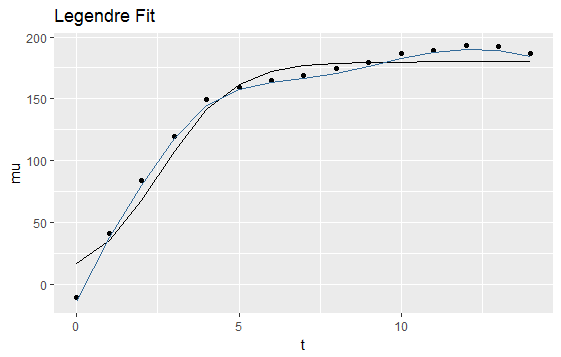
\includegraphics[width=0.8\linewidth]{images/LegendreFit} 

}

\caption{Additional Legendre Fit to Data}\label{fig:legendre-fit}
\end{figure}

As you can see from the step by step graphics, the mean growth curve is
fit. The example data follows the overall growth pattern but there is
some variation that is left to be explained. Each genetic marker is then
tested to see if the fit is improved by the addition of the effect
following the legendre polynomial. We see in the third graphic that the
selected line fits closer to the given data than using the mean growth
curve by itself. This genetic effect then would be selected and place
into the selection set. Further iterations to the procedure will then be
conducted to see if the fit can be further explained by the inclusion of
additional genetic or epistatic effects.

\section{Application}\label{application-2}

\subsection{Simulation Studies}\label{simulation-studies-1}

As statistical issues become more complex they are going to be more
analytically intractable and computational methods will need to close
that gap to show the effectiveness of new models and procedures.
Simulation studies were performed to ascertain the validity of the
model. Rates at which correct markers/epistasis were selected and
overall model true model size was assessed. Data was original generated
from a mean curve following the growth equation described above. It was
then sampled from a multivariate normal distribution with the mean
vector following the generated curve and correlated errors over time.
Significant effects were also included in the model to simulate
different marker levels. These effects could be main effects of SNPs, or
epistatic effects of interaction between SNPs. There were a total of
four main effects and three interaction effects simulated. This
simulation was replicated 100 times and then the selection procedure was
implemented. It performed well with each of the replicates selecting all
main and interaction effects that were set to be significant in the
underlying model. There were additional effects selected up to 14\% of
the time. You can see this in the false positive rate of the model
predictors. The true model size was simulated to be of size seven and
this was obtained the large majority of the time. The average model size
of the replicates fit was around 13.5 which explains the 14\% false
positive rate. This would indicate some slight over-fitting but all
important effects were included in the model. Future considerations for
this area could be beneficial to obtaining less over fitting.

\begin{table}

\caption{\label{tab:Chap4SimResults}Simulation Results}
\centering
\begin{tabular}[t]{l|r|r|r|r}
\hline
Model & T1\_tpr & T1\_fpr & T2\_tpr & T2\_fpr\\
\hline
Model Predictors & 1.0000 & 0.1417 & 1.0000 & 0.0037\\
\hline
Polynomial Degree & 0.7125 & 0.0251 & 0.9667 & 0.0007\\
\hline
\end{tabular}
\end{table}

\subsection{Worked Example}\label{worked-example-1}

Comparing to previous work in \ref{highorder} the same mei tree dataset
used in this chapter was reanalyzed. This serves as a comparison to
previous performance and also to see if any new discoveries can be made
by incorporating the time component and fitting the growth parameters
simultaneously throughout the procedure. The previous model only fit one
parameter of the growth equation as a time and assessed the genetic
markers that had a significant impact of this parameter. The parameter
focused on was the rate parameter,r for the shoot height of the progeny.
The initial results running the analysis with a single predictor and
using the selection procedure are,

\begin{table}

\caption{\label{tab:Chap4Table2}Table 6 The detection of epistasis for the relative growth rate (r) of shoot length in the full-sib family of mei tree by a high-order epistatic model}
\centering
\begin{tabular}[t]{lrrrl}
\toprule
Coefficient & Estimate & SE & T.value & P.value\\
\midrule
(Intercept) & 0.16859 & 0.05801 & 2.906 & 0.00415 **\\
AATTC\_nn\_np\_2517\_a & 0.27773 & 0.04396 & 6.318 & 2.27e-09 ***\\
AATTC\_nn\_np\_2815\_a & 0.26382 & 0.05295 & 4.983 & 1.54e-06 ***\\
CATG\_nn\_np\_3479\_a & 0.20767 & 0.03467 & 5.990 & 1.23e-08 ***\\
CATG\_nn\_np\_1284\_a & 0.04522 & 0.04265 & 1.060 & 0.29055\\
\addlinespace
AATTC\_nn\_np\_2815\_a×AATTC\_lm\_ll\_3034\_a & 1.82572 & 0.17925 & 10.185 & < 2e-16 ***\\
AATTC\_nn\_np\_2815\_a×AATTC\_hk\_hk\_278\_a & 0.25935 & 0.03888 & 6.671 & 3.48e-10 ***\\
CATG\_lm\_ll\_3153\_a & 0.14877 & 0.03491 & 4.262 & 3.36e-05 ***\\
CATG\_nn\_np\_1284\_a×AATTC\_nn\_np\_554\_a & 0.22994 & 0.05104 & 4.505 & 1.23e-05 ***\\
AATTC\_nn\_np\_2815\_a.AATTC\_lm\_ll\_3034\_a×AATTC\_nn\_np\_1615\_a & -1.51714 & 0.19060 & -7.960 & 2.39e-13 ***\\
\addlinespace
AATTC\_nn\_np\_2815\_a×AATTC\_nn\_np\_929\_a & -0.30805 & 0.05477 & -5.624 & 7.57e-08 ***\\
AATTC\_hk\_hk\_479\_d & 0.16044 & 0.03443 & 4.660 & 6.37e-06 ***\\
AATTC\_nn\_np\_2517\_a×CATG\_hk\_hk\_648\_a & 0.14537 & 0.02840 & 5.118 & 8.33e-07 ***\\
\bottomrule
\end{tabular}
\end{table}

Simultaneously fitting the growth curve and allowing for a more flexible
genetic effect to be fit to the data are presented below. As you can see
there are overlapping markers identified in the models. This shows the
robustness of the new selection technique to be consistent with previous
models. You can also see that the fit of the overall model has also
increased. By including all effects at once, you gain more statistical
power and it boost the adjusted R square value from 0.71 to above 0.9.
This boost in model performance could be partially due to some
over-fitting like we observed in the simulation studies and therefore a
very strict bonferroni correction was implemented to assess whether
individual markers were truly significant. Even with a strict cut-off we
still observed 3 epistatic predictors to be highly significant. This
shows the importance of including such terms while performing such a
GWAS. The other area to note is the highly significant intercept term,
\(\mu(t)\), which in our case is the result of the growth curve fit
before implementing the selection procedure. This indicates also the
importance of including biologically relevant information in the model
to help better understand the genetic architecture being studied of the
phenotype.

\begin{table}

\caption{\label{tab:Chap4Results}Growth Height}
\centering
\begin{tabular}[t]{l|r|r|r|r}
\hline
Coefficient & Estimate & SE & T.value & P.value\\
\hline
mu\_t & 0.9846 & 0.0142 & 69.2890 & 0.0000\\
\hline
CATG\_lm\_ll\_2801\_a\_P0 & -18.3460 & 2.3306 & -7.8719 & 0.0000\\
\hline
CATG\_lm\_ll\_2801\_a\_by\_AATTC\_lm\_ll\_2056\_a\_P0 & 15.0998 & 2.7364 & 5.5181 & 0.0000\\
\hline
CATG\_lm\_ll\_2801\_a\_by\_AATTC\_nn\_np\_2246\_a\_P0 & 17.4473 & 2.5890 & 6.7389 & 0.0000\\
\hline
CATG\_nn\_np\_3635\_a\_P0 & 35.6463 & 2.4577 & 14.5041 & 0.0000\\
\hline
CATG\_nn\_np\_3635\_a\_by\_CATG\_lm\_ll\_2637\_a\_P0 & -20.8632 & 2.1622 & -9.6492 & 0.0000\\
\hline
AATTC\_lm\_ll\_2056\_a\_by\_CATG\_lm\_ll\_2801\_a\_by\_CATG\_nn\_np\_4200\_a\_P0 & 11.6351 & 2.9936 & 3.8866 & 0.0001\\
\hline
AATTC\_nn\_np\_2246\_a\_by\_AATTC\_nn\_np\_4205\_a\_by\_CATG\_lm\_ll\_2801\_a\_P0 & -22.1074 & 3.3058 & -6.6874 & 0.0000\\
\hline
CATG\_nn\_np\_3635\_a\_by\_AATTC\_nn\_np\_2292\_a\_P0 & -16.8444 & 2.0928 & -8.0488 & 0.0000\\
\hline
AATTC\_hk\_hk\_753\_d\_P0 & -13.8052 & 1.8007 & -7.6664 & 0.0000\\
\hline
AATTC\_hk\_hk\_753\_d\_by\_AATTC\_hk\_hk\_485\_a\_P0 & 18.9017 & 2.0761 & 9.1045 & 0.0000\\
\hline
CATG\_nn\_np\_3635\_a\_by\_CATG\_nn\_np\_3234\_a\_P0 & -7.2607 & 2.4541 & -2.9586 & 0.0031\\
\hline
AATTC\_hk\_hk\_753\_d\_by\_CATG\_nn\_np\_2208\_a\_P0 & 7.8192 & 2.2885 & 3.4167 & 0.0006\\
\hline
AATTC\_hk\_hk\_485\_a\_by\_AATTC\_hk\_hk\_753\_d\_by\_AATTC\_nn\_np\_3611\_a\_P0 & -15.9119 & 3.0362 & -5.2407 & 0.0000\\
\hline
CATG\_lm\_ll\_2801\_a\_by\_AATTC\_nn\_np\_3395\_a\_P0 & -13.7696 & 2.3020 & -5.9816 & 0.0000\\
\hline
CATG\_lm\_ll\_1732\_a\_P0 & -8.9870 & 2.5788 & -3.4849 & 0.0005\\
\hline
CATG\_lm\_ll\_1732\_a\_by\_AATTC\_nn\_np\_4608\_a\_P0 & 23.9765 & 2.7677 & 8.6631 & 0.0000\\
\hline
AATTC\_nn\_np\_4608\_a\_by\_CATG\_lm\_ll\_1732\_a\_by\_CATG\_nn\_np\_3543\_a\_P0 & -18.6126 & 3.3495 & -5.5569 & 0.0000\\
\hline
CATG\_lm\_ll\_789\_a\_by\_CATG\_nn\_np\_3234\_a\_by\_CATG\_nn\_np\_3635\_a\_P0 & -11.7958 & 2.8852 & -4.0884 & 0.0000\\
\hline
CATG\_lm\_ll\_1732\_a\_by\_AATTC\_lm\_ll\_2212\_a\_P0 & 8.1659 & 2.1777 & 3.7498 & 0.0002\\
\hline
CATG\_lm\_ll\_1732\_a\_by\_CATG\_nn\_np\_2948\_a\_P0 & 9.5687 & 2.3217 & 4.1214 & 0.0000\\
\hline
AATTC\_hk\_hk\_495\_a\_by\_CATG\_lm\_ll\_1732\_a\_by\_CATG\_nn\_np\_2948\_a\_P0 & -8.6498 & 2.1831 & -3.9622 & 0.0001\\
\hline
AATTC\_nn\_np\_4608\_a\_by\_CATG\_lm\_ll\_1732\_a\_by\_CATG\_lm\_ll\_2787\_a\_P1 & 14.2735 & 2.1351 & 6.6852 & 0.0000\\
\hline
\end{tabular}
\end{table}

\section{Discussion}\label{discussion-2}

Some possible areas of concern for fitting the genetic effects to the
polynomials could be that the effect does not conform to the polynomial
curve under consideration. This can be alleviated by using other types
of basis functions such as splines, but this would also cost a huge
amount in computational efficiency with such a high dimensional data
set. You need to be as efficient as possible when implementing a GWAS
style study with the inclusion of possible epistasis. False positives
could be of concern as well throughout the selection. The flexibility of
the model and the wide range of polynomial fits that are considered
could result in artifacts in the data to be picked up on. This is
partially alleviated by using improved selection criteria like the
\(BIC_2\) and also having stricter than conventional cut-off values for
significance testing. However these would still need to be assessed
further through computational techniques such as cross-validation and
bootstrapping. The selection procedure is effective as a screening tool
for exploratory data analysis and hypothesis generation. Lab
verification would be another area that would help validate the findings
even further. The comparison to previously run models is promising step
in assessing the validity of the model at hand.

The new model proposed has some very nice features and performs well in
the given application. Considering the complexity of working with high
dimensional data coupled with including epsitatic effects as well as a
functional component to the phenotype, it performs relatively
efficiently. Using generalize least squares type calculations aided in
this efficiency, while taking into account the correlation that would
naturally arise between the repeated measurements of the same trees over
time. This was enabled by the framing of the regression problem as a
linear combination of basis functions. The agreeable properties of
orthogonal polynomials helped ensure model assumptions are being met as
closely as possible in order to use the calculations. Also by including
the biologically meaningful logistic growth equations it helps fit a
baseline fit to the data and would better allow for individual genetic
effects to be found throughout the selection. These would of course have
to be lab verified in order to assess the true biological mechanisms at
play for the genetic control of the phenotype.

\chapter{Conclusions}\label{conclusions-1}

\section{Summary}\label{summary}

In my dissertation I have applied, adapted and extended the forward
selection procedure under the marginality assumption first proposed by
\cite{hao2014interaction}. This procedure is able to reduce the search
space substantially by making some reasonable assumptions about the data
and underlying biological structure. These assumptions can be relaxed a
little to broaden the scope of the search space if desired. The
procedure has been applied in both simulated and real datasets in all
areas of study. There are many advantages to using such a procedure with
some being it is a computationally efficient way for high dimensional
data situations that arise from high throughput data, especially when
considering epistasis between gene markers or other type of interaction
effects in the model. The search space is guided based off of commonly
used principles in model selection that are relevant in real world
situations. It is able to perform a GWAS with included epistatic
interactions a fairly quick manner.

The ability to relax these assumptions leads to a widened search space
but may decrease the speed of the algorithm. This will make the search
more comprehensive and able to pick up on effects that may have been
missed with stricter assumptions. One nice use for the procedure is the
ability to screen for complex scenarios that would be hard to find in a
lab setting otherwise. The screening lends itself to find previously
undiscovered effects but with the flexibility of the initial model,
false positive rates could be a concern and need to be taken into
consideration. Adjustment to the significance level and the model
selection criteria have been made to account for this. This would still
need to be followed up by independently checking with other datasets
and/or lab verification techniques.

\subsection{HighDeQTL}\label{highdeqtl-1}

In \protect\hyperlink{highdeqtl}{Chapter 02} the iFORM procedure was
introduced and explored. It showed many desirable properties for high
dimensional data analysis. Simulation studies were performed to assess
the properties and compare across other models. After simulations were
conducted a real world application was conducted on gene expression data
and conducting a GWAS to find eQTLs for the different genes. Using all
markers in a single model as well as the inclusion of the possibility to
include epistatic effects as eQTLs gave a novel take on the reanalysis
of the C Elegans dataset. As we have seen there are many advantages to
the approach but one limiting question presented was that the
restriction on epistatic effects may have been too restrictive. Using
the strong heredity principle may miss some interactions that could
occur between markers that have not yet been selected. Also only
considering interactions with markers at two loci instead of higher
orders could be limiting the search to fully explain the expression
profile.

\subsection{Higher Order Epistasis}\label{higher-order-epistasis-1}

In \protect\hyperlink{highorder}{Chapter 03} higher order epistasis was
focused on the help explain a larger proportion of the phenotypic
variation. Extending the iFORM procedure to open up the possibility of
higher order epistasis is pivotal in understanding complex traits. More
support is coming out that phenotypes that are controlled by a multitude
of genetic and epigenetic effects potential could come from effects
involving three or more loci (\cite{taylor2014genetic}). Given that this
is the case the procedure was extended and simulation studies were
conducted to see the affect on the properties of the procedure.
Different levels of heredity and different orders of interactions were
also assessed. Other types of interaction models were also presented for
comparison purposes. The iFORM procedure performed well in the
simulation studies and appeared to capture the relevant information from
the underlying models. A real world application was then presented on a
growth parameter of Mei trees. The difference in running the procedure
with the possibility of finding higher order epistasis allowed for a
much greater proportion the variance to be explained by the markers.
This was favorable for the inclusion of higher order effects and showed
promise for the model. The phenotype was a static growth parameter,
which was the rate at which the trees grew for each individual
observation. The growth was measured over time and then a growth curve
was fit for each tree. This was then used for the phenotype. This was a
good approach but it misses the repeated measures and possibly other
information that may have been present throughout the growth process.
Since this is the case a functional phenotype was considered to help
capture all relevant information.

\subsection{iForm Functional Mapping}\label{iform-functional-mapping}

In \protect\hyperlink{iformfunc}{Chapter 04} functional components were
also considered for the selection procedure. This increases the
computational complexity of the model and therefore decreases some
efficiency gains previously seen but is necessary to capture all
information. Using biologically relevant information to guide the
fitting of the model to a functional curve will help improve the
efficiency and relevance. Initially well established growth equations
were considered as a baseline for the underlying structure. The
procedure then performs a GWAS level analysis with considering epistatic
interactions throughout the process. The selection of the markers as
possible genetic and epigenetic effects follows in a similar fashion as
the iForm procedure. Additional aspects had to be accounted for the
functional response and growth curve. Again simulation studies were
performed and a real world application was conducted. A reanalysis of
the full Mei tree dataset used in chapter 3 was explored. Including the
functional valued phenotype gave new insight into the genetic control.

\section{Discussion}\label{discussion-3}

The selection procedures proposed attempt to address problems that are
complex and have many moving parts to the procedure. Using a flexible
model is very helpful to fulfill such requirements but this could lend
itself to be prone to over fitting at times if not well controlled.
Being aware of this factor is part of interpreting the model a
researcher would need to be aware of. Using stricter selection criteria
and corrections to multiple testing for significance is extremely
important. The main purpose is to use as a screening to guide future
research while considering the possibilities of epistatic effects and
accounting for the entire genetic architecture at one time. The
importance of such a procedure could be used to help guide research and
also find new discoveries into complex, multi-loci traits that would be
extremely difficult to find in just a lab setting alone.

There are many attractive properties that the iFORM procedure posses. It
is computationally efficient given the large and growing predictor space
it uses. Along with the computational advantages, the selection
procedures proposed have sure screening properties. This indicates that
all the important effects in the true model will be selected with
probability tending to one. It also only includes a small proportion of
effects based off of a designated criteria that can be set. This will
help with interpretability of the final output as well as controlling
for the possibility of overfitting the data. There is still much that
can be extended and explored by using this type of selection procedure
on a variety of settings and/or phenotypes.

\section{Future Steps}\label{future-steps}

\subsection{Aim 1}\label{aim-1}

Incorporating other curves for the mean response curve could help extend
and relate to other areas of biology that follow a functional trait.
There are also other types of orthogonal polynomials that could be
explored as well. Using others polynomials would allow for other fits to
the data that may be more applicable in other scenarios. Also using
other basis functions in general could open up opportunities for other
areas of application. There are many non-linear functions that could be
used besides a polynomial fit that may also explain the underlying
genetic effects over time for other situations.

\subsection{Aim 2}\label{aim-2}

Other interesting areas would be to consider different levels of
interactions with other omics data. The gene-gene interactions
considered are only a portion of the picture and this type of modeling
could also handle complex levels of interactions that occur in a
biological system. One area that I am particularly interested in
applying it to would be in methylation and its interaction with gene
expression. This level of interaction is very important and a selection
procedure like the one proposed could help screen and generate possible
effects for hypotheses to continue to look into. This does not have to
be restricted to just within the biological system under study. It would
also apply in gene-environment interactions. Environmental factors are
important areas that could vastly impact the development of a phenotype.
Having the interaction with environmental factors could open up further
avenues that able to previously be explored.

\subsection{Aim 3}\label{aim-3}

Statistical areas that could as be considered to extend the model would
be to include multivariate responses to the system. For example having
gene and protein expression being a bivariate response and to see how
genetic markers and epistasis between the markers would better predict
this scenario. It could take the correlation between the protein and
expression response variables into account. Other statistical
considerations would be to extend selection criteria to help further
reduce the possibility of false positives being selected given a growing
dataset like the one that occurs while dynamically including interaction
effects throughout the selection. Making the model even more
computational efficient would always be beneficial as well. The faster a
model can accurately run the more likely a researcher will be to use it.
It will also help process all the high throughput data that is being
constantly developed.

\subsection{Closing Remarks}\label{closing-remarks}

Continuing on, my aim would be to work with datasets of high dimensional
scale and incorporate the types of statistical methods mentioned and
machine learning techniques to aid in analysis. The results could help
gain larger insights into the genomic/epigenetic architecture of
biological systems. On top of the importance of a functional component
to the phenotype, considering other types of multivariate responses
would be interesting to study in context of such a system. Integrating
different level of omics data and the challenges that arise with such
complicated and large datasets has interested me throughout my work.
Translating such a complex system into usable information that can be
shared in order to prevent and fight disease would be ideal research.
This type of research would need both methodological development as well
as application of existing statistical and machine/deep learning
techniques to handle the magnitude of the problem.

\chapter{Appendix}\label{appendix}

This needs more work. Only includes first part of the appendix pdf

\begin{center} 
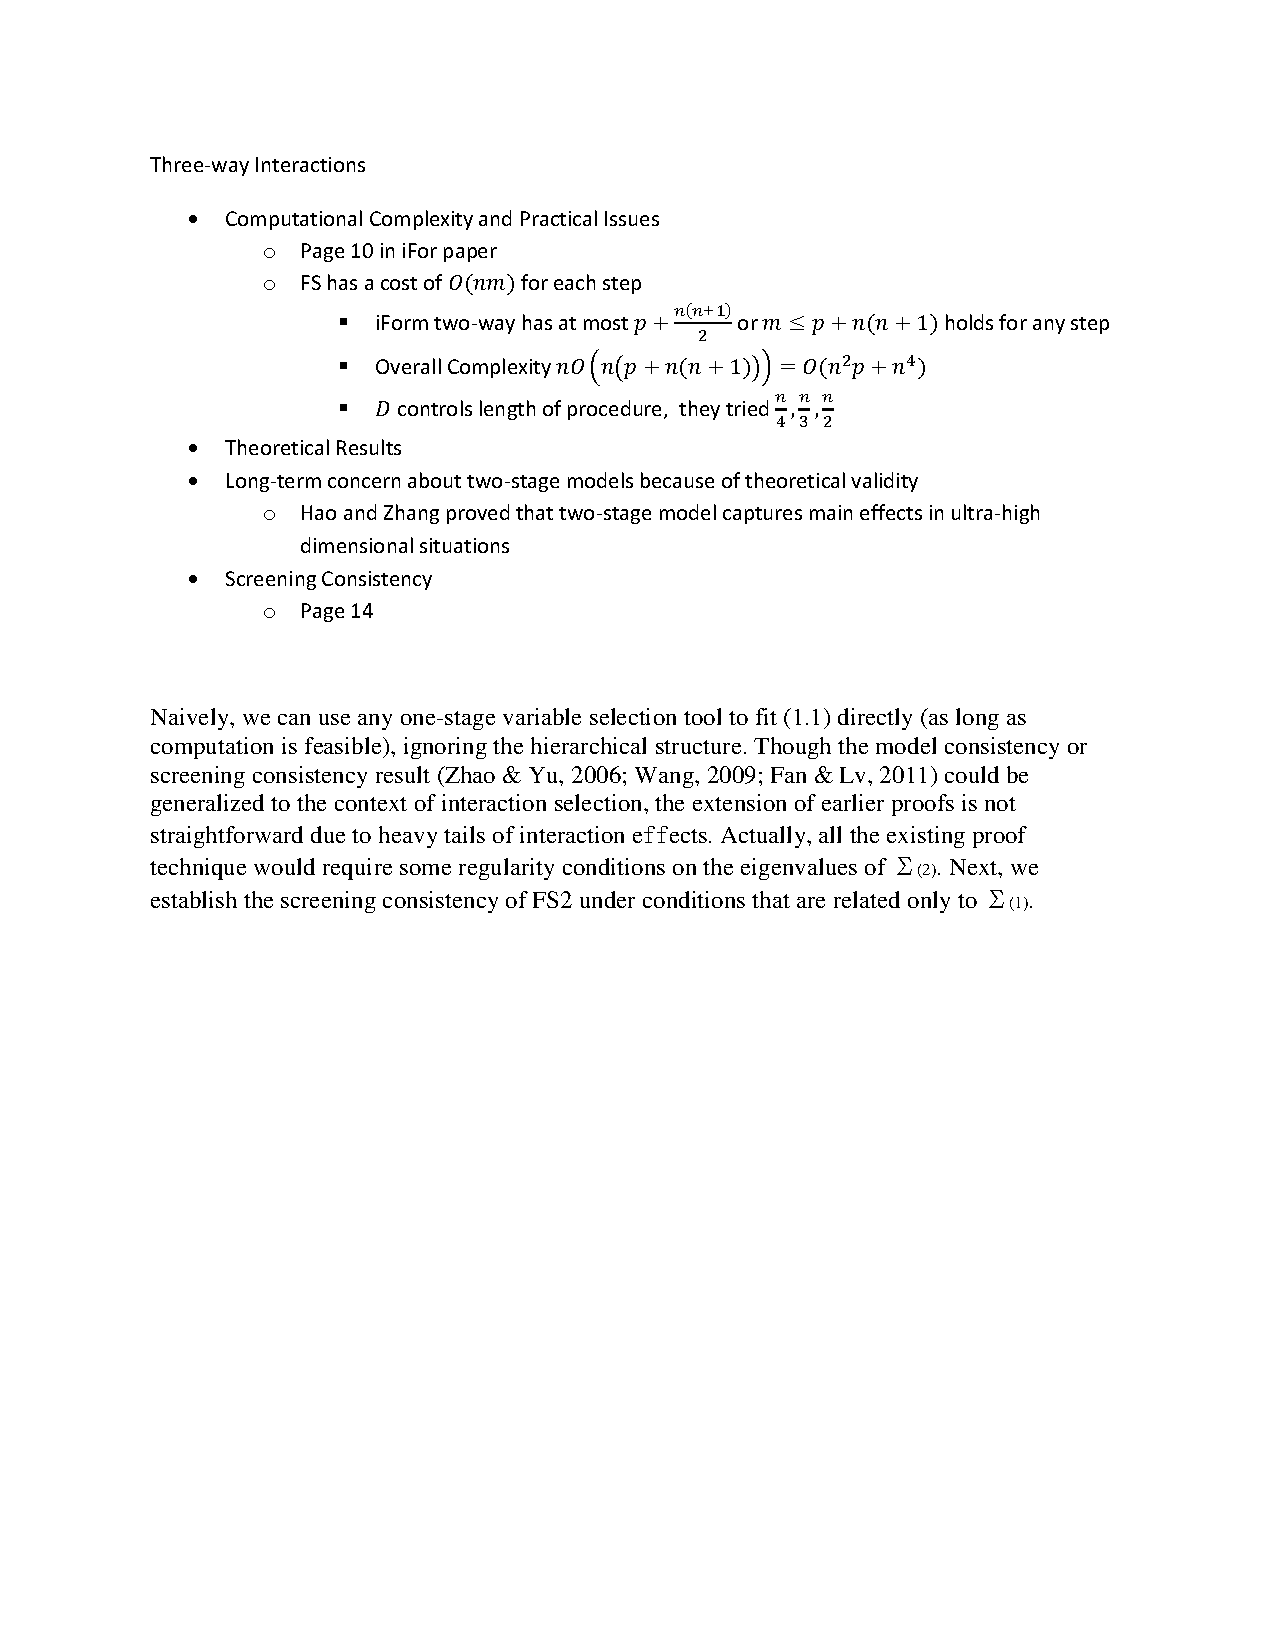
\includegraphics[width=8in]{appendix.pdf} 
\end{center}

\bibliography{packages,book}
\addcontentsline{toc}{chapter}{\bibname}


\end{document}
>>>>>>> b22dcdf6e44038e6b7615c4dec028252258563b2
